\documentclass[11pt,titlepage,twoside]{report}
\usepackage[T1]{fontenc}
\usepackage[utf8]{inputenc}
\usepackage{textcomp}

\usepackage[subdir=samples,
            prefix=tutorial,
            ext=.zls,
            prompt={aneto.local:\ },
            compiler={../compiler/zeluc.byte},
            compilerflags={-I ../lib -I ./samples},
            lastflags={-i},
            includecmd={},
           ]{runverbatim}
\fvset{xleftmargin=5mm}

\usepackage{a4wide}
\usepackage{hevea}
\usepackage{alltt}
\usepackage{url}
\usepackage{graphicx}
\usepackage{epsf}
\usepackage{amssymb}

\usepackage[printonlyused]{acronym}
% Put macro definitions below. Then, in the text write
%     \ac{ODE}      to use an acronym (the first use is expanded with the
%                   full definition),
%     \acp{ODE}     as above, but plural,
%     \acl{ODE}     show the full text,
%     \acs{ODE}     show just the short text,
%     etcetera. For more details, see page 2 of: 
%     ftp://ftp.tex.ac.uk/tex-archive/macros/latex/contrib/acronym/acronym.pdf
\acrodef{ODE}{Ordinary Differential Equation}
\acrodef{DAE}{Differential Algebraic Equation}
\acrodef{SSA}{Single Static Assignment}

\usepackage[inline]{enumitem}
\newlist{inparaenum}{enumerate*}{1}
\setlist[inparaenum,1]{label=(\arabic*),ref=\arabic*}
\newenvironment{flatitemize}
  {\begin{itemize}[leftmargin=*]}
  {\end{itemize}}

\usepackage{tikz}
\usetikzlibrary{positioning,chains,matrix,shapes.arrows,scopes,
                shapes.misc,arrows,automata,calc,decorations.markings}
\everymath{\displaystyle}
\tikzstyle{block} = [draw,fill=blue!20,minimum size=1.5em]
\tikzstyle{signal} = [draw,-latex,thick]
\tikzstyle{jump over} = [{to path={-- ([yshift=-.7mm]\tikztostart |- #1)
                          arc(-90:90:.7mm) |- (\tikztotarget)}}]

% see: 
% http://tex.stackexchange.com/questions/6135/how-to-make-beamer-overlays-with-tikz-node
\tikzset{onslide/.code args={<#1>#2}{%
  \only<#1>{\pgfkeysalso{#2}} % \pgfkeysalso doesn't change the path
}}

\tikzset{dimmedmarker/.code args={<#1> then <#2>}{%
  \alt<#1,#2>
  {
    \tikzstyle{marker} = [draw]
    \alt<#2>
    {\pgfkeysalso{->,red!80,draw opacity=.15}}
    {\pgfkeysalso{->,red!80,draw opacity=.50}}
  }
  {
    \tikzstyle{marker} = [draw=none]}
}}

\tikzset{zdimmedmarker/.code args={<#1> then <#2>}{%
  \alt<#1,#2>
  {
    \tikzstyle{marker} = [draw]
    \alt<#2>
    {\pgfkeysalso{->,blue!80,draw opacity=.15}}
    {\pgfkeysalso{->,blue!80,draw opacity=.50}}
  }
  {
    \tikzstyle{marker} = [draw=none]}
}}

\tikzstyle{every picture}+=[remember picture]
\tikzstyle{na} = [baseline=-.5ex]
\tikzstyle{ln} = [baseline,every node/.style={anchor=base,inner sep=0}]
\tikzstyle{lm} = [baseline,every node/.style={anchor=base}]

\tikzstyle{weak} =
  [decoration={markings,
               mark=at position -.6mm with {\draw[fill=white] circle (.6mm);},
               mark=at position -1.1mm with {\arrow{latex}},
              }, postaction={decorate}]

\tikzstyle{strong} =
  [decoration={markings,
               mark=at position .6mm with {\draw[fill=white] circle (.6mm);},
                  }, postaction={decorate}, -latex]
\newenvironment{hgraphicscope}[2]
  {
    \node[anchor=south west,inner sep=0] (image) at (0,0)
       {\includegraphics[width=#1]{#2}};
    \begin{scope}
    \tikzset{every node/.style={}, every path/.style={}}
    \clip (image.south west) rectangle (image.north east);
    \path let \p1=(image.south east) in (\y1, \x1) coordinate (ylimit);
    \end{scope}
    \begin{scope}[x={(image.south east)},y={(ylimit)},scale=0.1,]
  }
  {
    \end{scope}
  }

\tikzset{appear/.code args={<#1>}{%
  \pgfkeysalso{fill=gray!10,draw=gray!50,text=gray!50}
  \pgfkeysalso{pin edge={latex-,color=gray!50,thick}}
  \only<#1->{\pgfkeysalso{fill=blue!10,draw=black,text=black}}
  \only<#1->{\pgfkeysalso{pin edge={color=black,latex-,thick}}}
  \only<#1>{\pgfkeysalso{fill=red!50,draw=black,text=black}}
}}

\tikzset{text appear/.code args={<#1>}{%
  \pgfkeysalso{text=gray!50}
  \only<#1->{\pgfkeysalso{text=black}}
}}

\tikzset{line appear/.code args={<#1>}{%
  \pgfkeysalso{color=gray!50}
  \only<#1->{\pgfkeysalso{color=black}}
}}

%\usepackage[bookmarks, pagebackref, colorlinks, linkcolor=blue]{hyperref}

\long\def\framed#1{\framebox[\textwidth]{\vbox{\begin{center}#1\end{center}}}}
%utiliser \framed{...}

\newcommand{\zelus}{{\sf Z\'elus}}
\newcommand{\lucid}{{\sf Lucid}}
\newcommand{\lustre}{{\sf Lustre}}
\newcommand{\lucy}{{\sf Lucid Synchrone}}
\newcommand{\simulink}{{\sf Simulink}}
\newcommand{\stateflow}{{\sf Stateflow}}
\newcommand{\modelica}{{\sf Modelica}}
\newcommand{\scade}{{\sf SCADE}}
\newcommand{\scadesix}{{\sf SCADE~6}}
\newcommand{\esterel}{{\sf Esterel}}
\newcommand{\signal}{{\sf Signal}}
\newcommand{\statecharts}{{\sf StateCharts}}
\newcommand{\camllight}{{\sf Caml Light}}
\newcommand{\ocaml}{{\sf OCaml}}
\newcommand{\standardml}{{\sf Standard-ML}}
\newcommand{\lazyml}{{\sf Lazy-ML}}
\newcommand{\haskell}{{\sf Haskell}}
\newcommand{\ml}{{\sf ML}}
\newcommand{\inria}{{\sf INRIA}}
\newcommand{\alt}{\;|\;}

\newcommand{\zelusc}{\mbox{{\tt lucyc}}}

\newcommand{\AndEq}[2]{{#1}\,\mbox{{\tt and}}\,{#2}}

\newcommand{\Let}{\mbox{{\tt let}}}
\newcommand{\Rec}{\mbox{{\tt rec}}}
\newcommand{\In}{\mbox{{\tt in}}}
\newcommand{\And}{\mbox{{\tt and}}}
\newcommand{\Const}{\mbox{{\tt const}}}
\newcommand{\Fun}{\mbox{{\tt fun}}}
\newcommand{\Node}{\mbox{{\tt node}}}
\newcommand{\Emit}{\mbox{{\tt emit}}}
\newcommand{\Function}{\mbox{{\tt function}}}
\newcommand{\Arrow}{\mbox{{\tt ->}}}
\newcommand{\If}{\mbox{{\tt if}}}
\newcommand{\Then}{\mbox{{\tt then}}}
\newcommand{\Else}{\mbox{{\tt else}}}
\newcommand{\Merge}{\mbox{{\tt merge}}}
\newcommand{\Not}{\mbox{{\tt not}}}
\newcommand{\Pre}{\mbox{{\tt pre}}}
\newcommand{\Last}{\mbox{{\tt last}}}
\newcommand{\Run}{\mbox{{\tt run}}}
\newcommand{\Await}{\mbox{{\tt await}}}
\newcommand{\Fby}{\mbox{{\tt fby}}}
\newcommand{\When}{\mbox{{\tt when}}}
\newcommand{\Whenot}{\mbox{{\tt whenot}}}
\newcommand{\Extend}{\mbox{{\tt extend}}}
\newcommand{\Minusgreater}{\mbox{{\tt ->}}}
\newcommand{\Equalgreater}{\mbox{{\tt =>}}}
\newcommand{\Reset}{\mbox{{\tt reset}}}
\newcommand{\Every}{\mbox{{\tt every}}}
\newcommand{\Nil}{\mbox{{\tt Nil}}}
\newcommand{\Semisemi}{\mbox{{\tt ;;}}}
\newcommand{\On}{\mbox{{\tt on}}}
\newcommand{\Clock}{\mbox{{\tt clock}}}

\newcommand{\Where}{\mbox{{\tt where}}}
\newcommand{\Leq}{\mbox{{\tt <=}}}
\newcommand{\Le}{\mbox{{\tt <}}}
\newcommand{\Geq}{\mbox{{\tt >=}}}
\newcommand{\Ge}{\mbox{{\tt >}}}
\newcommand{\Neq}{\mbox{{\tt <>}}}
\newcommand{\Add}{\mbox{{\tt +}}}
\newcommand{\Mult}{\mbox{{\tt *}}}
\newcommand{\Or}{\mbox{{\tt or}}}
\newcommand{\Minus}{\mbox{{\tt -}}}
\newcommand{\Div}{\mbox{{\tt /}}}
\newcommand{\Mod}{\mbox{{\tt mod}}}
\newcommand{\false}{\mbox{{\em false}}}
\newcommand{\true}{\mbox{{\em true}}}
\newcommand{\End}{\mbox{{\tt end}}}

\newcommand{\DotNotation}[1]{\frac{\mathit{d}{#1}}{\mathit{dt}}}

\newcommand{\Nat}{I\!\!N}
\newcommand{\bR}{\mathbb{R}}
\newcommand{\bB}{\mathbb{B}}
\newcommand{\bN}{\mathbb{N}}

\newcommand{\Match}[2]{\mbox{\tt match}\ #1\ \mbox{\tt with}\ #2 \End}
\newcommand{\Automaton}[1]{\mbox{\tt automaton}\ {#1} \End}
\newcommand{\Present}[1]{\mbox{\tt present}\ {#1} \End}
\newcommand{\Until}{\mbox{\tt until}}
\newcommand{\Unless}{\mbox{\tt unless}}
%\newcommand{\Then}{\mbox{\tt then}}
\newcommand{\Continue}{\mbox{\tt continue}}
\newcommand{\Do}{\mbox{\tt do}}
\newcommand{\Done}{\mbox{\tt done}}

\newenvironment{paulo}{{\bf Paulo}}{{\bf fin Paulo}}
\newenvironment{marc}{{\bf Marc}}{{\bf fin Marc}}
\newenvironment{tim}{{\bf Tim}}{{\bf fin Tim}}

\newcommand{\Marc}[1]{{\bf Marc.} ({#1})}
\newcommand{\Tim}[1]{{\bf Tim.} ({#1})}

% Pour le manuel de ref
\newcommand{\term}[1]{{\tt #1}}
\newcommand{\nterm}[1]{{\em #1}}

% Un environnement pour les chronogrammes
\newenvironment{chrono}[1]
  {\begin{divstyle}{chrono}\center\tabular{#1}}
  {\endtabular\endcenter\end{divstyle}}

%\newenvironment{sample}
%  {\begin{flushleft} \begin{tabular}{p{.0cm}l}
%   &\begin{minipage}[t]{10cm} \begin{alltt}} {\end{alltt}
%   \end{minipage} \end{tabular}\end{flushleft}}

\newenvironment{sample}
  {\begin{flushright}\begin{minipage}[t]{15cm}\begin{alltt}}
  {\end{alltt}\end{minipage}\end{flushright}}

\newcommand{\shell}[1]{{\em aneto.local: #1}}
\newcommand{\sig}[1]{{\em #1}}

\begin{document}

\pagestyle{empty}

% we make a special title page for HeVeA
\begin{latexonly}
\vfill

\noindent {\huge \bf Z\'elus: a Hybrid Synchronous Language} \\[2ex]
{\Large Release, version 1.0}


\vspace{7cm}

\begin{center}
{\Huge \bf Tutorial and Reference Manual} \\

\vspace{1cm}
{\Large \url{http://zelus.di.ens.fr}}
\vspace{1.5cm}

{\Large Timothy Bourke and Marc Pouzet} \\[2ex]
{\large EPI PARKAS, DI and INRIA, \\
\'Ecole normale sup\'erieure, \\ 45 rue d'Ulm,
75230 Paris, France} \\[2ex]
{\Large January 2014} \\

\end{center}
% \vfill
% {\small \begin{verbatim}
% $Id: manual.tex,v 1.12 2009-02-08 11:15:55 pouzet Exp $
% \end{verbatim}}
\end{latexonly}
\begin{rawhtml}
  <div class="subtitle">Zelus</div>
  <div class="titlenote">Release, version 3.0</div>
  <div class="titlenote">Tutorial and Reference Manual</div>
  <div class="author">Marc Pouzet</div>
  <div class="date">May 2013</div>
\end{rawhtml}


\newpage
\cleardoublepage
\tableofcontents
\cleardoublepage

\chapter*{Foreword}

This document describes \zelus, a synchronous language extended with 
\acp{ODE} to model reactive systems where
discrete-time and continuous-time dynamics interact with each
other. A typical example is that of a software controller running in
closed loop with a physical environment. The language allows for
discrete and continuous-time dynamics to be modeled in the very same
program, and to generate sequential code which is paired with a
numeric solver for the \ac{ODE} part. \zelus{} shares the basic principles
of the synchronous language \lustre~\cite{lustre:ieee91} with several
of the features which were present in
\lucy~\cite{lucy:iste07}\footnote{\url{http://www.di.ens.fr/~pouzet/lucid-synchrone}}
(type inference, causality and initialization analyses, support for freely 
mixing data-flow equations and automata). The main features of the langage 
are:
\begin{flatitemize}
\item
The language is \emph{data-flow} and \ac{SSA}: every name has a single 
definition in the source code at at any instant. A program is a collection 
of function definitions that
transform signals into signals. A \emph{signal} is a function from a
time index to a set of values. A set of signals is defined uniquely as
the solution of a set of mutually recursive equations. The syntax of
\zelus{} is borrowed from \lucy~\cite{lucy:manual06}, although it is not 
completely backward compatible; for example, the syntax of automata has been 
modified to allow actions on transitions.
\item
Two kinds of signals are provided: discrete-time signals and
continuous-time signals.
\item
Discrete-time signals are \emph{infinite sequences} (or
\emph{streams}) of values like in other synchronous languages. Time
is thus logical, that is, we abstract from the amount of physical time that 
elapses between two successive values and treat signals as successions of 
values in a sequence.
A system is modeled
as a function that transforms streams into streams. \zelus{} is a
conservative extension of an existing synchronous language. Given the
main function of the system, the compiler produces a \emph{step}
function that computes a single reaction of the system and which is 
guaranteed
to run in bounded time and memory provided functions imported from the host 
language also do so.
\item
It is possible to mix discrete-time signals with continuous-time
ones defined by \acp{ODE}. Those
equations can be mutually recursive and/or depend on other stream
equations. Moreover, as for \simulink, \acp{ODE} can be reset when events 
occur. Currently, an event is either
\begin{inparaenum}
\item
the result of \emph{zero-crossing} detection, occurring when a 
continuous-time signal crosses zero from a negative value to a positive one 
during integration,
\item
the deadline of a \emph{timer}, which is a particular case
  of a zero-crossing event but which is implemented more efficiently using 
  horizons that limit the length of an integration phase, or,
\item
emitted from within a discrete expression.
\end{inparaenum}

\item
Abstract types,
product types, record types, and enumerated types can either be defined 
directly or imported
from the host language (\ocaml). Functions can have a polymorphic type 
\emph{à
  la ML}. Structured values can be accessed via pattern matching.
\item
The language allows the arbitrary composition of data-flow equations and 
hierarchical
automata with various forms of transitions. Compared to \stateflow,
these automata are safer in the sense that the compiler ensures the absence 
of both critical races (determinacy) and infinite loops.
Hierarchical
automata are rewritten into data-flow
equations and statically scheduled to generate sequential code.
\item
The compiler is written in \ocaml{} and is structured as a series of
source-to-source and traceable transformations that ultimately yield
statically scheduled sequential code written in \ocaml.
The results of intermediate steps can be written to output.
Continuous components are simulated using off-the-shelf
numerical solvers (here SUNDIALS
CVODE\footnote{\url{https://www.llnl.gov/casc/sundials/}}) and, currently
two built-in solver implementations (based on Matlab's \texttt{ode23} and
\texttt{ode45} solvers~\cite{ShampineRei:MatlabODE:1997}).
\end{flatitemize}

\zelus{} is a \emph{research prototype} for experimenting with new
techniques for building hybrid modelers; for example, the combination of
\simulink{} with \stateflow{} and \modelica{} on top of a synchronous
language. It currently only provides \acp{ODE} and not \acp{DAE} as
\modelica{} does. The language exploits novel techniques for defining
the semantics of hybrid modelers based on \emph{non-standard
  analysis}~\cite{lucy:jcss12}. It provides dedicated type systems to
ensure the absence of discontinuities during integration and the
generation of sequential code. In particular, all discrete
computations must be aligned to zero-crossing
events~\cite{lucy:lctes11,lucy:emsoft11}. The compiler is built on two
other type-based compile-time static analyses: programs with causality
loops which cannot be statically scheduled are
rejected~\cite{lucy:hscc14}; programs whose behavior depends on
uninitialized delays are statically rejected~\cite{lucy:sttt04}. These two
analyses conservatively extend earlier experiments in
the \lucy{} compiler.

\section*{Availability}
The implementation is written in, and generates programs in, \ocaml, which 
must be installed.
\begin{center}
\begin{tabular}{ll}
\zelus, version 1.0:  & 
  \ahrefurl{\url{http://zelus.di.ens.fr}} \\
Objective Caml, version 4.01  & 
  \ahrefurl{\url{http://www.ocaml.org}}
\end{tabular}
\end{center}
The language is experimental and evolves continuously. Please send
comments or bug reports to \url{Timothy.Bourke@inria.fr} or 
\url{Marc.Pouzet@ens.fr}. 

\section*{Copyright notice}
This software includes the \ocaml{} run-time system, which is
copyrighted INRIA, 2014. 

\section*{Thanks}
This software is a research prototype that takes considerable time to 
develop. If
you find it useful, please send us comments and cite it!
Currently, the best reference for \zelus{} is~\cite{lucy:hscc13}.

\cleardoublepage
\part{The Z\'elus Language}
\cleardoublepage

\chapter{Synchronous Programming}
\label{chapter:synchronous-programming}
%HEVEA\cutdef[1]{section}
The following two chapters are a tutorial introduction to \zelus. This
chapter focuses on the synchronous kernel of the language, reminiscent
of \lustre{} and \lucy. Every time possible, we shall point-out the
differences with those two languages. We devote the treatment of
continuous-time behaviors expressed by \acp{ODE} to
Chapter~\ref{chapter:ode-programming}. Chapter~\ref{chapter:complete-examples}
gathers some complete (but small) examples to figure out how
compilation proceeds.

A good familiarity with general programming
languages is assumed. Some familiarity with (strict or lazy) ML
languages and with existing synchronous data-flow languages is
helpful but not mandatory. Some references are given at the end of this document.

For this tutorial, we suppose that programs are written in a file
\verb-tutorial.zls-. This file is available in the \zelus{} distribution.

\section{The Core Synchronous Language}
%We start with the synchronous part of the language. \acp{ODE} and all 
%continuous
%aspect are considered later.

\subsection{Point-wise Operations}
The language is a first-order functional language. As in \lustre,
every ground type or any scalar value imported from the host language
\ocaml{} is implicitly lifted to signals. A signal is a \emph{stream}
of values, sequentially ordered in time, so that a value at an instant
cannot be produced if all the values at previous instants cannot have
been produced. This property models \emph{causality}. Thus:
\begin{itemize}
\item \verb-int- stands for the type of streams of integers,
\item \verb-1- stands for the  constant stream of values $1$,
\item \verb-+- adds point-wisely its two input streams. It can be seen
  as an adder circuit, in the same way, \verb-&- can be seen as an
  ``and'' gate. \\
\end{itemize}
Program executions can be represented as {\em chronograms}, showing
the sequence of values taken by streams during the execution. The
example below shows five streams, one per line. The first line shows
the value of a stream {\tt c}, which has the value $t$ ({\em true}) at the
first instant, $f$ ({\em false}) at the second one, and $t$ at the
third. The notation \dots indicates that the stream has more values
(it is infinite), not represented here. Similarly, the following lines
define {\tt x} and {\tt y}. The fourth line define a stream obtained
by adding {\tt x} and {\tt y}, addition is done point-wisely.

\begin{chrono}{c|cccc}
\hline
\tt c & $t$ & $f$ & $t$ & \dots \\ \hline
\tt x & $x_0$ & $x_1$ & $x_2$ & \dots \\ \hline
\tt y & $y_0$ & $y_1$ & $y_2$ & \dots \\ \hline 
\tt x+y & $x_0+y_0$ & $x_1+y_1$ & $x_2+y_2$ & \dots \\ \hline 
\tt if c then x else y &  $x_0$ & $y_1$ & $x_2$ & \dots \\ \hline
\end{chrono}

\subsection{Delays}

{\tt fby} is a delay operator. The expression {\tt x fby y}, which can
be read as ``{\tt x} {\em followed by} {\tt y}'' takes the first value
of {\tt x} at the first instant, then takes the previous value of {\tt
  y}. In other words, it delays {\tt y} by one instant, and is
initialized by {\tt x}. This operator is borrowed from the language
\lucid~\cite{lucida}.
\begin{chrono}{c|cccc}
\hline
\tt x & $x_0$ & $x_1$ & $x_2$ & \dots \\ \hline
\tt y & $y_0$ & $y_1$ & $y_2$ & \dots \\ \hline 
\tt x fby y &  $x_0$ & $y_0$ & $y_1$ & \dots \\ \hline
\end{chrono}
It is often needed to separate the delay from the initialization. This
is done using the delay operator {\tt pre}, and the initialization
operator {\tt ->}. {\tt pre x} delays its argument {\tt x}, and has an
unspecified value (denoted here by {\em nil}) at the first
instant. {\tt x -> y} takes the first value of x at the first instant,
then the current value of y. The expression {\tt x -> (pre y)} is
equivalent to {\tt x fby y}.
\begin{chrono}{c|cccc}
\hline
\tt x & $x_0$ & $x_1$ & $x_2$ & \dots \\ \hline
\tt y & $y_0$ & $y_1$ & $y_2$ & \dots \\ \hline 
\tt pre x &  $nil$ & $x_0$ & $x_1$ & \dots \\ \hline 
\tt x -> y &  $x_0$ & $y_1$ & $y_2$ & \dots \\ \hline
\end{chrono}
The {\em initialization check} made by the compiler checks that the
behavior of a program never depends on the value {\em nil}. See
section~\ref{initialisation-check} for details.

\medskip\noindent{\bf Warning:} A common error with the initialization
operator is to use it for defining the first two values of a
stream. This does not work, since \verb+x -> y -> z+ =
\verb+x -> z+. One should instead write \verb-x fby y fby z- or,
\verb+x -> pre (y -> pre z)+. E.g., the stream which starts with value
$1$ and is followed by $2$ and $3$ forever is written: \verb-1 fby 2 fby 3-
or \verb+1 -> pre(2 -> pre(3))+ or \verb+1 -> pre(2 -> 3)+.

\subsection{Global declarations}
A program is made of a sequence of declarations of global
values. \verb-let- defines non recursive global values. These global values may
be constant or functions. For example:
\begin{runverbatim}
let dt = 0.001
let g = 9.81
\end{runverbatim}
These declarations define two infinite constant streams \verb-dt- and
\verb-g-. Once typed, the compiler displays their type using the option {\tt -i}:
\begin{sample}\runverbatimcmd\end{sample}
\runverbatimmsg
For each declaration, we get the inferred type.
Only constant values can be defined globally, thus rejecting the
following program:
\begin{runverbatim}[fail]
let first = true -> false
\end{runverbatim}
Trying to compile this program, we get the following answer:
\begin{sample}\runverbatimcmd\end{sample}
\runverbatimerr
The right part of a global \verb-let- declaration cannot contain any
delay operations. Definitions containing delays can only be under the
definitions of a {\tt node} definition (see~\ref{sec:sequential-functions}).

\subsection{Combinatorial Functions}
Signal functions are separated into {\em combinatorial} and {\em
sequential} functions. A function is combinatorial when its output at
instant $n$ depends only on its input at the same instant $n$.

The definition of combinatorial function uses the {\tt let} notation
seen previously. Consider, for example, the function computing the
average of its two inputs. We directly give its type
signatures as computed by the compiler.
\begin{runverbatim}[withresult]
let average (x,y) = (x + y) / 2
\end{runverbatim}
This function get the type signature \verb+int * int -A-> int+ stating
that it takes two integer streams and returns an integer stream. The
tagged arrow \texttt{-A->} with mark \texttt{A} indicates that
\texttt{average} is combinatorial. \texttt{A} means ``any'', that is,
\texttt{average} can be used anywhere in the code. This will be
detailled further.

Function definition can contain local declarations, introduced using
either the {\tt where}, or the {\tt let} notation
(see~\ref{sec:local-defin-mutu}). For example the average function can
be written in two (equivalent) manners:
\begin{runverbatim}
let average (x,y) = o where o = (x + y) / 2
\end{runverbatim}
\begin{runverbatim}
let average (x,y) =
  let o = (x + y) / 2 in o
\end{runverbatim}

As another example of combinatorial program, we end with the classical
description of a one-bit adder. A full adder takes three bits
(\verb-a-, \verb-b- and a carry bit \verb-c-) and it returns the
result \verb-c- and the new carry \verb-co-.
\begin{runverbatim}[withresult]
let xor (a, b) = (a & not(b)) or (not a & b)
let full_add(a, b, c) = (s, co) where
   rec s = xor (xor (a, b), c)
   and co = (a & b) or (b & c) or (a & c)
\end{runverbatim}

\begin{figure}
\begin{center}
\begin{tabular}{ll}
%BEGIN IMAGE
\includegraphics[width=0.3\textwidth]{Fig/half_adder}
%END IMAGE
%HEVEA\imageflush
& \quad\quad
%BEGIN IMAGE
\includegraphics[width=0.5\textwidth]{Fig/full_adder}
%END IMAGE
%HEVEA\imageflush
\end{tabular}
\end{center}
\caption{A half-adder and a full-adder~\label{half-adder}}
\end{figure}

A full adder can be described more efficiently as a composition
of two half adders. The graphical description is given in
figure~\ref{half-adder} and it corresponds to the following code:
\begin{runverbatim}[continue,withresult]
let half_add(a,b) = (s, co) where
   rec s = xor (a, b)
   and co = a & b
\end{runverbatim}

\begin{runverbatim}[continue,withresult]
let full_add2(a, b, c) = (s, co) where
  rec (s1, c1) = half_add(a,b)
  and (s, c2) = half_add(c, s1)
  and co = c1 or c2
\end{runverbatim}

\subsection{Sequential Functions}
\label{sec:sequential-functions}
Sequential functions (or state functions) are such that their output
at instant $n$ may depend on the history of their inputs, that is,
input values of instants $k$ ($k \leq n$). An expression is called
sequential if it may produce a time evolving value when its free
variables are kept constant.  Otherwise, we call it combinatorial. A
sufficient condition to be a combinatorial expression is not to
contain any delay, initialization operator, nor automaton.

Sequential functions are introduced by the keyword \verb-node-. They receive
a different type signature than the one given to combinatorial functions.
The type signature \texttt{int -D-> int} states that \verb-from- is
a stream function from an integer stream to an integer stream and
that its output may depend on the history of its input. 

The following function computes the sequence of integers starting at
some initial value given by parameter \verb-m-:
\begin{runverbatim}[withresult]
let node from m = nat where
  rec nat = m -> pre nat + 1
\end{runverbatim}
Applying this function to the constant stream {\tt 0} yields the
following execution:
\begin{chrono}{l|ccccccc}
\hline
\tt m                 & $0$ & $0$ & $0$ & $0$ & $0$ &  $0$ & \dots \\ \hline
\tt 1                 & $1$ & $1$ & $1$ & $1$ & $1$ &  $1$ & \dots \\ \hline
\tt pre nat           & $nil$ & $0$ & $1$ & $2$ & $3$ &  $4$ & \dots \\ \hline
\tt pre nat + 1       & $nil$ & $1$ & $2$ & $3$ & $4$ &  $5$ & \dots \\ \hline
\tt m -> pre nat + 1  & $0$ & $1$ & $2$ & $3$ & $4$ &  $5$ & \dots \\ \hline
\tt from m            & $0$ & $1$ & $2$ & $3$ & $4$ &  $5$ & \dots \\ \hline
\end{chrono}

Combinatorial functions are checked to be combinatorial at compile
time, thus forgetting the keyword \verb-node- leads to an error:
\begin{runverbatim}[fail]
let from n = nat where
  rec nat = n -> pre nat + 1
\end{runverbatim}
and we get:
\begin{sample}\runverbatimcmd\end{sample}
\runverbatimerr
Whereas it is not possible to call a node (arrow type \texttt{-D->})
in a combinatorial function, it is possible to do the converse: to
call a combinatorial function (arrow type \texttt{-A->}) in a
node. E.g., the addition called in function \texttt{from} has type
signature: \texttt{int * int -A-> int}.

\medskip\noindent
The edge front detector is defined in the following way:
\begin{runverbatim}
let node edge c = c & not (false fby c)
\end{runverbatim}
\begin{chrono}{l|ccccccc}
\hline
\tt c                 & $f$ & $f$ & $t$ & $t$ & $f$ &  $t$ & \dots \\
\hline
\tt false             & $f$ & $f$ & $f$ & $f$ & $f$ &  $f$ & \dots \\
\hline
\tt false fby c       & $f$ & $f$ & $f$ & $t$ & $t$ &  $f$ & \dots \\
\hline
\tt not (false fby c) & $t$ & $t$ & $t$ & $f$ & $f$ &  $t$ & \dots \\
\hline
\tt edge c            & $f$ & $f$ & $t$ & $f$ & $f$ &  $t$ & \dots \\
\hline
\end{chrono}
\noindent \verb-edge- is a global function from boolean streams to
boolean streams. 

\medskip\noindent
An Euler forward integrator is defined by:
\begin{runverbatim}[withresult,label=integr]
let dt = 0.01
let node integr (x0, x') = x where
  rec x = x0 -> pre (x +. x' *. dt)
\end{runverbatim}
\verb-integr- is a global function returning a stream \verb-x- defined
recursively so that, for all $n \in \Nat, x(n) = x0 + \sum_{i=0}^{n-1}
x'(i)\cdot dt$.  The operators \verb-+.-, \verb-*.- stand for the
addition and multiplication over floating point numbers. Sequential
functions may be composed as any other functions. For example:
\begin{runverbatim}[continue]
let node double_integr (x0, x0', x'') = x where
  rec x = integr (x0, x')
  and x' = integr (x0', x'')
\end{runverbatim}

% \subsection{Anonymous Functions}
% Functions can be defined in an anonymous way and can be used as
% values. Anonymous combinatorial functions are introduced using a
% single arrow ({\tt ->}), anonymous sequential ones using a double
% arrow ({\tt =>}). For example, the expression \verb#fun x y -> x + y#
% is the sum function and has type \verb#int -> int -> int#). The
% expression \verb#fun x y => x fby x fby y# defines a double delay and
% has the type \verb#'a -> 'a => 'a#.

% The functions \verb-average- and \verb-from- can be defined as:
% \begin{runverbatim}
% let average = fun (x,y) -> (x + y) / 2
% let from = fun n => nat where rec nat = n -> pre nat + 1
% \end{runverbatim}

\subsection{Local Definitions and Mutually Recursive Definition}
\label{sec:local-defin-mutu}
Variables may be defined locally with a \verb-let/in- or
\verb-let rec/in- and there is no special restriction on the
expressions appearing on the right of a definition. The following
program, computes the Euclidean distance between two points:

\begin{runverbatim}
let distance ((x0,y0), (x1,y1)) =
  let d0 = x1 -. x0 in
  let d1 = y1 -. x1 in
  sqrt (d0 *. d0 +. d1 *. d1)
\end{runverbatim}
Notice that because \verb-d0- and \verb-d1- denote infinite streams
the computations of \verb+x1 -. x0+ and \verb+y1 -. x1+ are
(virtually) executed in parallel.  Nonetheless, when writing sequences
of definitions \verb-let/in- such as above, the sequential order is
preserved for each reaction of the system, that is, the current value
of \verb-d0- is always computed before the current value of
\verb-d1-. The preservation of the sequential order is useful when functions
with side-effects are imported from the host language. If you do not want to
specify any order, write \texttt{let rec d0 = ... and d1 = ...} instead.

Streams may be defined as a set of mutually recursive equations.  The
function which computes the minimum and maximum of an input stream
\verb-x- can be written in the three equivalent manners:
\begin{runverbatim}
let node min_max x = (min, max) where
  rec min = x -> if x < pre min then x else pre min
  and max = x -> if x > pre max then x else pre max
\end{runverbatim}

\begin{runverbatim}
let node min_max x =
  let rec min = x -> if x < pre min then x else pre min
  and max = x -> if x > pre max then x else pre max in
  (min, max)
\end{runverbatim}

\begin{runverbatim}
let node min_max x = (min, max) where
  rec (min, max) = (x, x) -> if x < pre min then (x, pre max)
                             else if x > pre max then (pre min, x)
                             else (pre min, pre max)
\end{runverbatim}

\noindent The classical sinus and cosinus functions can be defined like the
following:
\begin{runverbatim}[continue,include=integr]
let node sin_cos theta = (sin, cos) where
  rec sin = integr(0.0, theta *. cos)
  and cos = integr(1.0, -. theta *. sin)
\end{runverbatim}

We end with the programming of a mouse controller, a very
classical example. Its specification is the following:
\begin{quote}
Return the event \verb-double- when two \verb-click- has been received
in less than four \verb-top-. Emits \verb-simple- if only one click
has been received.
\end{quote}
Here is a possible implementation:
\begin{runverbatim}
(* counts the number of events from the last reset res *)
let node counter (res,event) = count where
  rec count = if res then 0 else x
  and x = 0 -> if event then pre count + 1 else pre count

let node mouse (click,top) = (single,double) where
  rec counting = click -> if click & not (pre counting) then true
                          else if res & pre counting then false
                          else pre counting
  and count = counter(res,top & counting)
  and single = ((0 fby count) = 3) & top & not click
  and double = (false fby counting) & click
  and res = single or double
\end{runverbatim}

\subsection{Shared Memory and Initialization}
The language provides an alternative way to the use of the delay
\verb-pre- in order to refer to the previous value of a stream. If
\verb-o- is a stream variable defined by some equation, \verb-last o-
refers to the last value of \verb-o-. For example:
\begin{runverbatim}
let node counter i = o where
  rec init o = i
  and o = last o + 1
\end{runverbatim}
The equation \verb-init o = i- defines the initial value of the {\em
  memory} \verb-last o-. This memory is initialized with the first
value of \verb-i- and then, contains the previous value of
\verb-o-. The above program is thus equivalent to the following
one:\footnote{The construction \texttt{last} is eliminated during the
  compilation process by a similar transformation.}
\begin{runverbatim}
let node counter i = o where
  rec last_o = i -> pre o
  and o = last_o + 1
\end{runverbatim}
The memory \verb-last o- will play an important role when combined
with control structures. This will be illustrated later.
From a syntactical point of view, \verb-last- is {\em not} an
operator: \verb-last o- denotes a shared memory and the argument of
\verb-last- is necessarily a name. Thus the following program:
\begin{runverbatim}[fail]
let node f () = o where
  rec o = 0 -> last (o + 1)
\end{runverbatim}
is rejected and we get:
\runverbatimerr

Instead of defining the current value of a signal according to its previous
values, it is also possible to define the next value according to the current
one. The counter
can also be defined in the following ways:

\begin{runverbatim}
let node counter i = o where
  rec init o = i
  and next o = o + 1
\end{runverbatim}
or:
\begin{runverbatim}
let node counter i = o where
  rec next o = o + 1 init i
\end{runverbatim}
In the two definitions, \texttt{o} is initialized with the very first value of
\verb-i- and the value of \texttt{o} at instant $n+1$ equals the value of
\texttt{o+1} at instant $n$ (for all $n \in \Nat$).

None of the two forms --- defining the current value of a signal
according to its previous value \emph{versus} defining the next value
according to the current one --- is better than the other. Both are
equivalent in the sense that one can be transformed into the
other. This depend on the situation. Nonetheless, we shall see in
Section~\ref{chapter:ode-programming} that restrictions apply on the
use of the operator \texttt{last} when combining discrete-time and
continuous-time dynamics.

Currently, the compiler translates the
constructions \verb-last-, \verb+->+, \verb-fby- and \verb+pre+ into
a combination of \verb-init- and \verb-next-. E.g., the equation \texttt{x = pre(e)}
is translated into \texttt{next x = e}.

\subsection{Causality check}
\label{causality-check}
Recursively defined values must not contain any {\em instantaneous} or
{\em causality} loops in order to be able to generate statically schedulable
sequential code. For example, if we type:
\begin{runverbatim}[fail]
let node from m = nat where
  rec nat = m -> nat + 1
\end{runverbatim}
the compiler emits the message:
\runverbatimerr
This program cannot be computed as {\tt nat} depends on {\tt nat}
instantaneously.

The compiler statically reject function definitions which cannot be scheduled
sequentially, that is streams whose value at instant $n$ may depend on
some value at instant $n$. In practice, it imposes that any loop
crosses a delay \verb-pre- or \verb-fby-. This is the purpose of
the \emph{causality analysis} to reject such loops.

In the current version of the compiler, function definitions are
implicitly inlined at their call site. Note that delays can be hidden
internally in the body of a function as this is the case for the languages \lustre{}
and \signal, for example. E.g., the following function definition
which approximates the \ac{ODE} below
\[
\dot{t} = g_0 - g_1 \cdot t \quad t(0) = t_0
\]
by a difference equation is causally correct:

\begin{runverbatim}[withresult,include=integr]
(* [t0] is the initial temperature; [g0] and [g1] two constant *)
let node heater(t0, g0, g1) = t where
  rec t = integr(t0, g0 -. g1 *. t)
\end{runverbatim}
It is also possible to force
that a function be compiled once and turn into a single step function
which compute the current value of its outputs from the current value of its
inputs. This is specified by
adding the keyword \texttt{atomic}. E.g., the following program is now rejected
by the causality analysis.
%
\begin{runverbatim}[fail,withresult]
let atomic node f x = 0 -> pre (x + 1)
let node wrong () =
  let rec o = f o in o
\end{runverbatim}
%
Indeed, whereas the output
of \texttt{f} does not instantaneously depend on its input \texttt{x},
adding the keyword \texttt{atomic} forces to consider that all output
instantaneously depend on all inputs. For atomic functions, the
compiler produces a single step function which is simply
called.\footnote{Modular code generation where a function is split
  into a minimal set of functions, as proposed
  in~\cite{lucy:emsoft09,lustre:tripakis-popl09}, is not implemented
  in the current version of the compiler.}

\subsection{Initialization check}
\label{initialisation-check}
The compiler checks that every delay operator is initialized. For
example:
\begin{runverbatim}[fail,withresult]
let node from m = nat where
  rec nat = pre nat + 1
\end{runverbatim}
The analysis is a {\em one-bit} analysis where expressions are
considered to be either always defined or always defined except at the
very first instant.  It is defined in~\cite{lucy:sttt04}. In
practice, it rejects expressions like \verb-pre (pre e)-, that is,
un-initialized expressions cannot be used as an argument of a delay
and must be first initialized using \verb+->+.


\section{Data-types, Pattern matching}

\subsection{Type definitions}
Product types, record types and enumerated type may be defined in the same
way as in \ocaml. No sum type is provided at the moment. It is nonetheless
possible to define abstract types and to inport functions from an \ocaml{} module.
See the present reference manual for syntactic considerations.

Records are defined like in Ocaml and accessed with the dot notation. E.g.,
the following defines a type {\tt
  circle}, representing a circle as a record containing a {\tt
  center}, given by its coordinates, and a {\tt radius}.
\begin{runverbatim}
type circle = { center: float * float; radius: float }

let center c = c.center
let radius c = c.radius
\end{runverbatim}
  
\subsection{Pattern matching}
The language provides means for doing pattern matching over streams
with a \verb-match/with- construction {\em \`a la} \ocaml.

Consider the example of a colored wheel rotating on an axis and for
which we want to compute the rotation direction. This wheel is
composed of three sections with colors blue (\verb-Blue-), red
(\verb-Red-) and green (\verb-Green-).  A sensor observes the
successive colors on the wheel and has to decide if the wheel is
immobile or determine the rotation direction.

We consider that the direction is direct (\verb-Direct-) when there is
a succession of \verb-Red-, \verb-Green-, \verb-Blue-, \verb-Red-...,
the opposite direction being indirect (\verb-Indirect-). There are
some instants where the direction is undetermined
(\verb-Undetermined-) or that the wheel is immobile (\verb-Immobile-).

We program the controler in the following way. First, we introduce two
sum types.  The function \verb-direction- then compares three
successive values of the input stream \verb-i-.
\begin{runverbatim}
type color = Blue | Red | Green
type dir = Direct | Indirect | Undetermined | Immobile
\end{runverbatim}

\begin{runverbatim}[continue,withresult]
let node direction i = d where
  rec pi = i fby i
  and ppi = i fby pi
  and match ppi, pi, i with
    (Red, Red, Red) | (Blue, Blue, Blue) | (Green, Green, Green) ->
         do d = Immobile done
  | (_, Blue, Red) | (_, Red, Green) | (_, Green, Blue) -> 
         do d = Direct done
  | (_, Red, Blue) | (_, Blue, Green) | (_, Green, Red) -> 
         do d = Indirect done
  | _ -> do d = Undetermined done
  end
\end{runverbatim}

The handler of a pattern-matching construct is made of a set of
equations defining {\em shared} variables (here the variable
\verb-d-). At each instant, the \verb-match/with- statement selects
the first pattern (from top to bottom) which matches the actual value
of the triple \verb-pii, pi, i- and executes the corresponding
branch. During a reaction, only one branch is executed.

Because only one branch is executed during a reaction, one must be
careful when programming with such control structures, in particular
in the presence of delay operators. This can be illustrated on the
following program. This program is made of two modes: in the \verb-Up-
mode, the variable \verb-o- increases by step \verb-1- whereas in the
mode \verb-Down-, it decreases by step \verb+-1+.
\begin{runverbatim}
type modes = Up | Down

let node two (m, i) = o where
  rec init o = i
  and match m with
      | Up -> do o = last o + 1 done
      | Down -> do o = last o - 1 done
      end
\end{runverbatim}
The equation \verb-init o = i- defines a shared memory \verb-last o-
which is initialized with the first value of \verb-i-. \verb-o- is
called a shared variable because it is defined by several
equations. When \verb-m- equals \verb-Up-, \verb-o- equals
\verb-last o + 1-. When \verb-m- equals \verb-Down-, \verb-o- equals
\verb+last o - 1+.  The communication between the two modes is done
through a shared memory \verb-last o-.  \verb-last o- contains the
previous value of \verb-o-, the last time \verb-o- has been
defined. The execution diagram for some execution is given below.
\begin{chrono}{l|cccccccc}
\hline
\tt i                 & \tt 0  & \tt 0  & \tt 0 & \tt 0    & \tt 0  & \tt 0    &  \tt 0  & \dots \\
\hline
\tt m                 & \tt Up & \tt Up & \tt Up & \tt Down & \tt Up & \tt Down &  \tt Down & \dots \\
\hline
\tt last o + 1        & \tt 1  & \tt 2  & \tt 3  &          & \tt 3  &       & 
& \dots \\
\hline
\tt last o - 1        &        &        &        & \tt 2    &        & \tt 2 &  \tt 1   & \dots \\
\hline
\tt o                 & \tt 1  & \tt 2  & \tt 3    & \tt 2    & \tt 3  & \tt 2    &  \tt 1  & \dots \\
\hline
\tt last o            & \tt 0  & \tt 1  & \tt 2    & \tt 3  & \tt 2    &  \tt 3  & \tt 2 & \dots \\
\hline
\end{chrono}

\medskip\noindent
The function \texttt{two} is equivalent to the following one:
\begin{runverbatim}[hide,label=updownmodes]
type modes = Up | Down
\end{runverbatim}
\begin{runverbatim}[continue]
let node two (m, i) = o where
  rec last_o = i -> pre o
  and match m with
      | Up -> do o = last_o + 1 done
      | Down -> do o = last_o - 1 done
      end
\end{runverbatim}
making clear that \verb-last o- stands for the previous defined value
of \verb-o-.

\subsection{The Difference between Pre and Last}
Whereas \verb-last o- may seem
to be just another way to refer to the previous value of a stream like
\verb-pre o- does, there is a fundamental difference between the
two. This difference is a matter or instant of observation.

\begin{itemize}
\item
In block-diagram formalism {\em \`a la}
\simulink\ or \scade, $\texttt{pre}\;e$ is a unit delay which
is a local memory. $\texttt{pre}$ denotes the last value of its argument, the
last time it was {\em observed}. If $\texttt{pre}\;e$ appear in a
block structure which is executed from time to time --- say when some condition
$c$ is true --- it means that the argument $e$ is only computed when
$c$ is true.
\item
$\texttt{last}\;o$ denotes the previous value of the variable $o$ on
  the instant where the variable $o$ is {\em defined}.
  $\texttt{last}\;o$ is only valid when $o$ stands for a variable and
  not an expression.  $\texttt{last}\;o$ is useful to communicate
  values between modes and this is why we call it a shared memory.
\end{itemize}

We illustrate the difference between the two on the following
example. We now compute two other streams \verb-c1- and \verb-c2-
returning respectively the number of instants each mode is active.
\begin{runverbatim}[include=updownmodes]
let node two (m, i) = (o, c1, c2) where
  rec init o = i
  and init c1 = 0
  and init c2 = 0
  and match m with
       | Up -> do o = last o + 1
              and c1 = 1 -> pre c1 + 1
              done
       | Down -> do o = last o - 1
                 and c2 = 1 -> pre c2 + 1
                 done
    end
\end{runverbatim}

The equation \verb#c1 = 1 -> pre c1 + 1# is only active in the
\verb-Up- mode whereas equation \texttt{c2 = 1 -> pre c2 + 1} is
active in mode \verb-Down-. The execution diagram is given below.
\begin{chrono}{l|cccccccc}
\hline
\tt i                 & \tt 0  & \tt 0  & \tt 0 & \tt 0    & \tt 0  & \tt 0    &  \tt 0  & \dots \\
\hline
\tt m                 & \tt Up & \tt Up & \tt Up & \tt Down & \tt Up & \tt Down &  \tt Down & \dots \\
\hline
\tt last o + 1        & \tt 1  & \tt 2  & \tt 3  &          & \tt 3  &       & 
& \dots \\
\hline
\tt 1 -> pre c1 + 1   & \tt 1  & \tt 2  & \tt 3  &          & \tt 4  &       & 
& \dots \\
\hline
\tt last o - 1        &        &        &        & \tt 2    &        & \tt 2 &  \tt 1   & \dots \\
\hline
\tt 1 -> pre c2 + 1   &        &        &        & \tt 1    &        & \tt 2 &  \tt 3   & \dots \\
\hline
\tt o                 & \tt 1  & \tt 2  & \tt 3    & \tt 2    & \tt 3  & \tt 2    &  \tt 1  & \dots \\
\hline
\tt last o            & \tt 0  & \tt 1  & \tt 2    & \tt 3  & \tt 2    &  \tt 3  & \tt 2 & \dots \\
\hline
\tt c1                 & \tt 1  & \tt 2  & \tt 3    & \tt 3    & \tt 4  & \tt 4    &  \tt 4  & \dots \\
\hline
\tt c2                 & \tt 0  & \tt 0  & \tt 0    & \tt 1    & \tt 1  & \tt 2    &  \tt 3  & \dots \\
\hline
\end{chrono}

A pattern matching composes several complementary sub-streams.
The above pattern matching has
two branches. Every branch defines its own clock, one denoting the
instants where \verb-m = Up- and the other denoting the instant where
\verb-m = Down-.

\subsection{Local Definitions}
It is possible to define variables which stay local to a branch. For
example:

\begin{runverbatim}[include=updownmodes]
let node two (m, i) = o where
  match m with
  | Up -> let rec c = 0 -> pre c + 1 in
          do o = c done
  | Down -> do o = 0 done
  end
\end{runverbatim}
or equivalently:
\begin{runverbatim}[include=updownmodes]
let node two (m, i) = o where
  match m with
  | Up -> local c in
          do c = 0 -> pre c + 1 and o = c done
  | Down -> do o = 0 done
  end
\end{runverbatim}
In the first handler of the \texttt{match/with} statement, \texttt{c} is
declared to be local to the handler. The compiler checks that a definition for
\texttt{c} is given. Several variables can be declared local by writing
\texttt{local c1,..., cn in ...}.
\subsection{Implicit Completion of Shared Variables}
Finally, note that the branches of a pattern-matching constraint do
not have to contain a definition for all the shared variables. A
shared variable is implicitly completed as if one has written
equations of the form \verb-x = last x- in branches where no
definition for \verb-x- is given. Finally, the compiler rejects situations
where it is unable to ensure that an initial value exist for
\texttt{last x}. Thus, the following program is rejected.
\begin{runverbatim}[withresult,fail,include=updownmodes]
let node two (m, i) = o where
  rec match m with
      | Up -> do o = last o + 1 done
      | Down -> do o = last o - 1 done
      end
\end{runverbatim}

% \begin{verbatim}
% type event = Click | Move | Keypressed of char

% (* count the number of Move between two click *)
% let node count e = cpt where
%   rec last o = 0
%   and match e with
%         Top -> do o = last o + 1 done
%       | Click -> do o = last o done
%       end
% \end{verbatim}

% A pattern matching composes several complementary sub-streams, that
% is, streams on complementary clocks. The above pattern matching 
% has two branches. Every branch defines its own clock, one denoting
% the instants where \verb-e = Top- and the other denoting the instant
% where \verb-e = Click-.

% The branch \verb#Top when clk -> (pre o) when clk + 1#
% states that for the instants where the condition \verb-e = Top- is
% true (\verb-clk- being the clock of this branch), the result is the
% previous value of \verb-o- plus one. For the instants where
% \verb-e = Click-, the result is \verb-0-.

% The pattern-matching construction is very similar to the \verb-merge-
% construction and thus, benefit (and somethimes suffers ?) from the same clock
% constraints. Thus, writing simply \verb-(pre o) + 1- would lead to a
% clocking error since \verb-o- is on the base clock and must be sampled
% on the clock of the branch.

% The execution diagram is given below.

% \vspace{.5cm}

% \begin{tabular}
% {c|ccccccc}
% \hline
% \tt e                 & \tt Click & \tt Top & \tt Top & \tt Click & \tt Top &  \tt Click & \dots \\
% \hline
% \tt clk		      & $f$   & $t$ & $t$ & $f$   & $t$ &  $f$ & \dots \\
% \hline
% \tt Top when clk      &       & \tt Top & \tt Top &       & \tt Top &      & \dots \\
% \hline
% \tt (pre o) when clk + 1
%                       &       & $1$ & $2$ &       & $1$ &      & \dots \\
% \hline
% \tt Click             & \tt Click   &   &  & \tt Click   &   &  \tt Click & \dots \\
% \hline
% \tt 0                 & $0$   &  &  & $0$   &  &  $0$ & \dots \\
% \hline
% \tt o                 & $0$   & $1$ & $2$ & $0$   & $1$ &  $0$ & \dots \\
% \hline
% \end{tabular}

% \vspace{.5cm}

% This program can also be written in the following way:
% \begin{verbatim}
% let count e =
%   let rec o =
%     0 -> match e, pre o with
%       Top, o -> o + 1
%     | _ -> 0 in
%   o
% \end{verbatim}

% If we get back to the first version of the \verb-count- function, the reader may
%  notice the difference between an expression
% \verb-(pre o) when clk- which refers to ``the value of \verb-o- at the last
% global instant'' and \verb-pre (o when clk)- which refers ``the value
% of \verb-o- at the last instant where \verb-clk- was true''. To illustrate
% this difference, consider now the problem of counting the distance
% made by a mouse between two clicks.

% \begin{verbatim}
% (* computes the distance between two click *)
% let distance pos_x e =
%   0 -> match e with
%     Click when c -> pos_x when c - pre (pos_x when c)
%   | Top -> 0

% (* second way *)
% let distance d e =
%   0 -> match e, d with
%     Click, d -> d - pre d
%   | _ -> 0
% \end{verbatim}
% The execution diagram is given below.

% \vspace{.5cm}

% \begin{tabular}
% {c|ccccccc}
% \hline
% \tt pos\_x                 & $1$       & $2$     & $3$     & $3$       & $3$ &  $5$ & \dots \\
% \hline
% \tt e                 & \tt Click & \tt Top & \tt Top & \tt Click & \tt Top &  \tt Click & \dots \\
% \hline
% \tt Click when c      & \tt Click   &  & & \tt Click      & &  \tt Click  & \dots \\
% \hline
% \tt pos\_x when c     & $1$       &     &     & $3$       &  &  $5$ & \dots \\
% \hline
% \tt pre (pos\_x when c) & $nil$   &     &     & $1$       &  &  $3$ & \dots \\
% \hline
% \tt pos\_x when c -
% pre (pos\_x when c)      & $nil$  &     &     & $2$       &  &  $2$ & \dots \\
% \hline
% \tt distance d e       & $0$       & $0$&     & $2$        & $0$ & $2$ & \dots \\
% \hline
% \end{tabular}

% \vspace{.5cm}
% The \verb-match/with- construction is a generalised form of
% \verb-merge-. These constructions are the natural way to express
% control structure in a data-flow language. In the example above, the
% computation  
% \verb+pos_x when c - pre (pos_x when c)+ is only executed when
% \verb-e- equals \verb-Click-. The compilers deeply rely on clocks for
% generating good imperative code.

\section{Valued Signals}
\label{signals}
The language provides a way to manage {\em valued signals}. Signals
are built and accessed through the constructions \verb-emit- and
\verb-present-.  At every instant, a value signal is a pair made of (1) a boolean
$c$ indicating when the signal is present and (2) a value present when $c$ is
true.\footnote{For \ocaml{} programmers, a signals correspond to a value
of an option type.}
 
\subsection{Signal Emission}
As opposed to shared variables, it is now possible to give a partial definition
with no implicit completion. Consider the following program:
\begin{runverbatim}[withresult]
let node within (min, max, x) = o where
  rec c = (min <= x) & (x <= max)
  and present c -> do emit o = () done
\end{runverbatim}
It computes a condition \verb-c-. Then \verb-o- is a signal
which is present, an receive the value \verb-()- every time \verb-c- is
true. There is no need here to give an initial value to \verb-o-. When \verb-c- is
false, \verb-o- is simply absent.

\subsection{Testing the Presence of a Signal and Accessing its Value}
It is possible to test for the presence of a signal expression $e$ by
writing the boolean expression $? e$. The following program, for
example, counts the number of instants where \verb-x- is emitted.
\begin{runverbatim}[withresult]
let node count x = cpt where
  rec cpt = if ?x then 1 -> pre cpt + 1 else 0 -> pre cpt
\end{runverbatim}

The language provides a more general mechanism to test for the
presence of several signals and access their values. It is reminiscent
of the pattern-matching construct of ML.  This pattern matching
mechanisn is safe in the sense that it is possible to access the value
of a signal only at the instant where it is emitted.\footnote{This
  contrasts the \esterel{} solution where the value of a signal
  implicitly holds and can be accessed even when it is not
  emitted. This restriction may appear cumbersome in some situation
  but it is safer. In particular, it avoids initialization issues and
  avoid the need to allocate a state variable to store the previous
  value as needed otherwise.}

The following program takes two signals \verb-x- and \verb-y- and
returns an integer which equals the sum of \verb-x- and \verb-y- when
both are emitted, it returns the value of \verb-x- when \verb-x- is
emitted only and the value \verb-0- when only \verb-y- is emitted and
\verb-0- otherwise.
\begin{runverbatim}[withresult]
let node sum (x, y) = o where
  present
  | x(v) & y(w) -> do o = v + w done
  | x(v1) -> do o = v1 done
  | y(v2) -> do o = v2 done
  else do o = 0 done
  end
\end{runverbatim}
A \verb-present- statement is made of several signal conditions and
handlers. Each condition is tested sequentially. The signal condition
\verb-x(v) & y(w)- is verified when both signals \verb-x- and \verb-y-
are present. A condition \verb-x(v1)- means ``\verb-x- is present and
has some value \verb-v1-''. The variable \verb-v1- can in turn be used
in the corresponding handler. The last signal condition \verb-_-
stands for the wildcard signal condition which is always verified.

In the signal pattern \verb-x(v) & y(w)-, \verb-x- and \verb-y- are
expressions evaluating to signal values whereas \verb-v- and \verb-w-
stand for patterns. Thus, writing \verb-x(42) & y(w)- would mean:
``await for the presence of signal \verb-x- evaluating to \verb-42-
and the presence of \verb-y-.

Note that the output of the function \verb-sum- is a regular flow
since the test is exhaustive. Forgetting the default case will raise
an error.
\begin{runverbatim}[withresult,fail]
let node sum (x, y) = o where
  present
  | x(v) & y(w) -> do o = v + w done
  | x(v1) -> do o = v1 done
  | y(v2) -> do o = v2 done
  end
\end{runverbatim}

We can easily eliminate this error by giving a last value to \verb-o-
(e.g., adding an equation \verb-init o = 0- outside of the present
statement). In that case, the default case is implicitly completed
with an equation \verb-o = last o-. The other way is to state that
\verb-o- is now a signal and is thus only partially defined.
\begin{runverbatim}[withresult]
let node sum (x, y) = o where
  present
  | x(v) & y(w) -> do emit o = v + w done
  | x(v1) -> do emit o = v1 done
  | y(v2) -> do emit o = v2 done
  end
\end{runverbatim}

A signal pattern may also contain boolean expressions. The following
program, sums the values of the two signals \verb-x- and \verb-y-
provided they arrive at the same time and \verb-z >= 0-.
\begin{runverbatim}
let node sum (x, y, z) = o where
  present
    x(v) & y(w) & (z >= 0) -> do o = v + w done
  else do o = 0 done
  end
\end{runverbatim}

\medskip\noindent{\bf Remark:} Using signals, we can mimic the
\verb-default- construction of the language
\signal. \verb-default x y- emits the value of \verb-x- when \verb-x-
is present and the value of \verb-y- when \verb-x- is absent and
\verb-y- is present. The signal pattern \verb+x(v) | y(v)+ tests the
presence of ``\verb-x- or \verb-y-''.
\begin{runverbatim}
let node default (x, y) = o where
  present
    x(v) | y(v) -> do emit o = v done
  end
\end{runverbatim}
This is, of course, only a simulation since all the information about
the precise instants where \verb-x- and \verb-y- are present --- the
so-called \emph{clock calculus} --- are hidden at run-time and not exploited
by the compiler. In particular,
the compiler is unable to state that \verb-o- is emitted only when
\verb-x- or \verb-y- are present as the clock calculus of
\signal~\cite{signal:pldi} does for the default operator.

The current version of \zelus{} does not provide a \emph{clock calculus} as
\lustre, \lucy{} and \signal{} do.

\section{Hierarchical State Machines}
The language provides means to define state machines, as a way to
describe directly control dominated systems. These state machines can
be composed in parallel with regular equations or other state machines
and can be arbitrarily nested. State machines are essentially borrowed
\emph{as is} from \lucy{} and their
\scadesix~\footnote{\url{http://www.esterel-technologies.com/products/scade-suite/}}version.

In this tutorial, we first consider state machines where transitions
are only made of boolean expressions. Then, we consider two important
extensions of the basic model. The first one is the ability to build
define state machines with parameterized states and actions on
transitions. The second one introduces the general form of transitions
made of signal matching and boolean expressions.

An automaton is a collection of states and transitions. Two kinds of
transitions are provided, namely {\em weak} and {\em strong}
transitions and for each of them, it is possible to enter in the next
state by {\em reset} or by {\em history}. One important feature of
these state machines is that {\em only one set of equations is
  executed during one reaction}.

\subsection{Strong Preemption}
Here is a two state automaton illustrating strong preemption. The
function \verb-expect- awaits \verb-x- to be true and emits
\verb-true- for the remaining instants.
\begin{runverbatim}[withresult]
(* await x to be true and then sustain the value *)
let node expect x = o where 
  automaton
  | S1 -> do o = false unless x then S2
  | S2 -> do o = true done
  end
\end{runverbatim}

This automaton is made of two states, each of them defining the value
of a {\em shared} variable \verb-o-. The keyword \verb-unless-
indicates that \verb-o- is defined by the equation \verb-o = false-
from state \verb-S1- while \verb-x- is false. At the instant where
\verb-x- is true, \verb-S2- becomes the active state for the remaining
instant. Thus, the following chronogram hold:
\begin{chrono}{c|ccccccc}
\hline
\tt x                 & \tt false & \tt false & \tt true & \tt false & \tt false &  \tt true & \dots \\
\hline
\tt expect x           & \tt false & \tt false & \tt true & \tt true & \tt true &  \tt true & \dots  \\ \hline
\end{chrono}

\subsection{Weak Preemption}
On the contrary, the following function emits \verb-false- at the
instant where \verb-x- is true and \verb-true- for the remaining
instants, thus corresponding to regular {\em Moore automata}.
\begin{runverbatim}[withresult]
(* await x to be true and then sustain the value *)
let node expect x = o where 
  automaton
  | S1 -> do o = false until x then S2
  | S2 -> do o = true done
  end
\end{runverbatim}

\begin{chrono}{c|ccccccc}
\hline
\tt x                 & \tt false & \tt false & \tt true & \tt false & \tt false &  \tt true & \dots \\
\hline
\tt expect x           & \tt false & \tt false & \tt false & \tt true & \tt true &  \tt true & \dots  \\ \hline
\end{chrono}

The classical two states \verb-switch- automaton can be written like
the following:
\begin{runverbatim}
let node weak_switch on_off = o where
  automaton
  | False -> do o = false until on_off then True
  | True -> do o = true until on_off then False
  end
\end{runverbatim}

Note the difference with the following form with weak transitions only:
\begin{runverbatim}[continue]
let node strong_switch on_off = o where
  automaton
  | False -> do o = false unless on_off then True
  | True -> do o = true unless on_off then False
  end
\end{runverbatim}

We can check that for any boolean stream \verb-on_off-, the following
property holds:
\begin{runverbatim}[continue,skipone]
let node correct on_off =
weak_switch on_off = strong_switch (false -> pre on_off)
\end{runverbatim}
The graphical representation of these two automata is given in
figure~\ref{switch-figure}.

\begin{figure}
%BEGIN IMAGE
\begin{center}
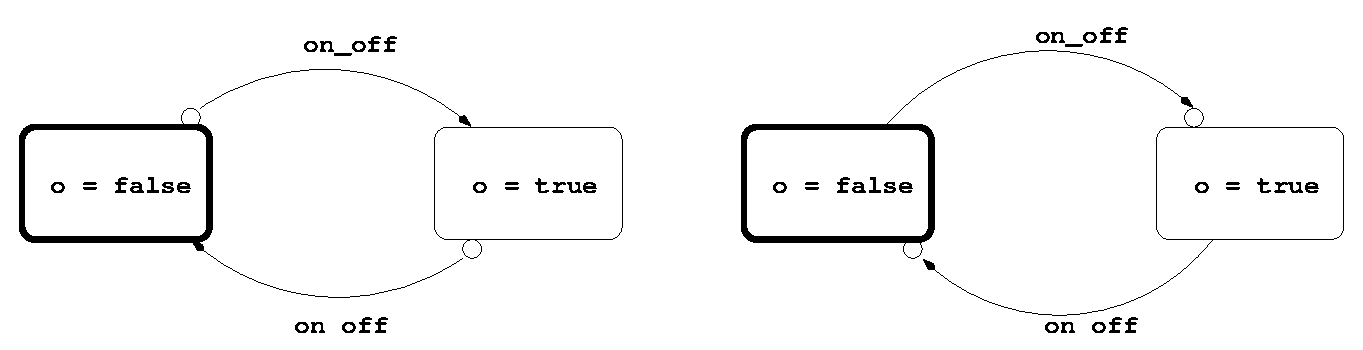
\includegraphics[width=\textwidth]{Fig/automaton}
\end{center}
%END IMAGE
%HEVEA\imageflush
\caption{Two automata with strong and weak transitions~\label{switch-figure}}
\end{figure}

Weak and strong conditions can be arbitrarily mixed as in the
following variation of the switch automaton:
\begin{runverbatim}
let node switch2 (on_off, stop) = o where
  automaton
  | False -> do o = false until on_off then True
  | True -> do o = true until on_off then False unless stop then Stop
  | Stop -> do o = true done
  end
\end{runverbatim}

Compared to the previous version, state \verb-True- can be strongly
preempted when some stop condition \verb-stop- is true.

\subsection{ABRO and Modular Reseting}
The ABRO example is due to G\'erard Berry~\cite{esterel:primer99}. It
highlight the expressive power of parallel composition and preemption
in Esterel. The specification is the following:

\begin{quote}
Awaits the presence of events \verb-A- and \verb-B- and emit \verb-O-
at the exact instant where both events have been received.  Reset this
behavior every time \verb-R- is received.
\end{quote}
Here is how we write it, replacing capital letters by small
letter~\footnote{As in \ocaml, identifiers starting with a capital
  letter are considered to be constructors and cannot be used for
  variables.}.

\begin{runverbatim}
(* emit o and sustain it when a and b has been received *)
let node abo (a, b) = (expect a) & (expect b)

(* here is ABRO: the same except that we reset the behavior *)
(* when r is true *)
let node abro (a, b, r) = o where
  automaton
    S1 -> do o = abo (a, b) unless r then S1
  end
\end{runverbatim}

The node \verb-abro- is a one state automaton which {\em resets} the
computation of \verb-abo a b-: every stream in \verb-abo a b- restarts
with its initial value. The language provides a specific
\verb-reset/every- primitive as a shortcut of such a one-state
automaton and we can write:

\begin{runverbatim}
let node abro (a, b, r) = o where
  reset
    o = abo (a, b)
  every r
\end{runverbatim}

The \verb-reset/every- construction combines a set of parallel
equations (separated with an \verb-and-). Note that the reset
operation correspond to strong preemption: the body is reseted at the
instant where the condition is true. The language does not provide a
``weak reset''. Nonetheless, it can be easily obtained by inserting a
delay as illustrated below.

\begin{runverbatim}
  let node abro (a, b, r) = o where
    reset
      o = abo (a, b)
    every true -> pre r
\end{runverbatim}

% It is also possible to write:

% \begin{verbatim}
% let node abro a b r = o where
%   rec automaton
%         S1 -> do automaton
%                    S1 ->
%                     do o = (except a) & (except b)
%                     until o then S2
%                  | S2 -> do o = true done
%                  end
%               unless r then S1
%       end
% \end{verbatim}

\Marc{Rajouter l'exemple de blink/blink.}

\begin{runverbatim}
let node blink_reset (r, n, m, t) = x where
 reset
   automaton
   | On  -> do x = true  until (after(n, t)) then Off
   | Off -> do x = false until (after(m, t)) then On
 every r
\end{runverbatim}

\medskip
The type signatures inferred by the compiler are:
\runverbatimmsg

\subsection{Local Definitions in a State}
It is possible to define names which are local to a state. These names
can only be used inside the body of the state and may be used in weak
conditions only.

The following programs integrates the integer sequence \verb-v- and
emits false until the sum has reached some value \verb-max-. Then, it
emits \verb-true- during \verb-n- instants.

\begin{runverbatim}
let node consume (max, n, v) = status where
  automaton
  | S1 ->
      let rec c = v -> pre c + v in
      do status = false
      until (c = max) then S2
  | S2 ->
      let rec c = 1 -> pre c + v in
      do status = true
      until (c = n) then S1
  end
\end{runverbatim}

State \verb-S1- defines a local variable \verb-c- which can be used to
compute the weak condition \verb-c = max- and this does not introduce
any causality problem. Indeed, weak transitions are only effective
during the next reaction, that is, they define the next state, not the
current one. Moreover, there is no restriction on the kind of
expressions appearing in conditions and they may, in particular, have
some internal state. For example, the previous program can be
rewritten as:

\begin{runverbatim}
let node counting v = cpt where
  rec cpt = v -> pre cpt + v

let node consume (max, n, v) = status where
  automaton
  | S1 ->
       do status = false
       until (counting v = max) then S2
  | S2 ->
       do status = true
       until (counting 1 = n) then S1
  end
\end{runverbatim}
The body of a state is a sequence (possibly empty) of local
definitions (with \verb-let/in-) followed by some definitions of
shared names (with \verb-do/until-). As said previously, weak
conditions may depend on local names and shared names.

It is important to notice that using \verb-unless- instead of
\verb-until- leads to a {\em causality error}. Indeed, in a strong
preemption, the condition is evaluated {\em before} the equations of
the body and thus, cannot depend on them. In a weak preemption, the
condition is evaluated at the end, {\em after} the definitions of the
body have been evaluated. Thus, when writing:

\begin{runverbatim}[fail]
let node consume (max, n, v) = status where
  automaton
  | S1 ->
      let rec c = v -> pre c + v in
      do status = false
      unless (c = max) then S2
  | S2 ->
      let rec c = 1 -> pre c + v in
      do status = true
      unless (c = n) then S1
  end
\end{runverbatim}
The compiler emits the message:
\runverbatimerr
%\begin{sample}
%File "tutorial.zls", line 6:
%> unless c = max then S2
%>        ^^^^^^^
%This expression may depend on itself.
%\end{sample}
\Tim{ Marc: ce programme n'est pas correct pour une mauvais raison: on ne 
peut pas lire un \texttt{c} local dans une transition forte! Alors que tu 
veux démontrer une problème de dépendance cyclique.}

\subsection{Communication between States and Shared Memory}
In the previous examples, there is no communication between values
computed in each state. Consider a simple system made of two running
modes as seen previously. In the \verb-Up- mode, the system increases
some value with a fixed step \verb-1- whereas in the \verb-Down- mode,
this value decreased with the same step. Now, the transition from one
mode to the other is described by a two-state automaton whose behavior
depends on the value computed in each mode. This example, due to
Maraninchi \& R\'emond~\cite{Modes-SCP03} can be programmed in the
following way.

\begin{runverbatim}[include=updownmodes]
let node two_states (i, min, max) = o where
  rec automaton
      | Up -> do o = last o + 1
              until (o = max) then Down
      | Down -> do o = last o - 1
                until (o = min) then Up
      end
  and init o = i
\end{runverbatim}
An execution diagram is given below:
\begin{chrono}
{l|ccccccccccccc}
\hline
\tt i                 & \tt 0  & \tt 0  & \tt 0 & \tt 0    & \tt 0  & \tt 0    &  \tt 0  & \tt 0  & \tt 0 & \tt 0    & \tt 0  & \tt 0   & \dots \\
\hline
\tt min               & \tt 0  & \tt 0  & \tt 0 & \tt 0    & \tt 0  & \tt 0    &  \tt 0  & \tt 0  & \tt 0 & \tt -1    & \tt 0  & \tt 0   & \dots \\
\hline
\tt max               & \tt 4  & \tt 4  & \tt 4 & \tt 4    & \tt 4  & \tt 4    &  \tt 4 & \tt 4  & \tt 4 & \tt 4    & \tt 4  & \tt 4    & \dots \\
\hline
\tt last o            & \tt 0 & \tt 1 & \tt 2 & \tt 3 & \tt 4 & \tt 3 &  \tt 2 
& \tt 1  & \tt 0 & \tt -1    & \tt 0  & \tt 1   & \dots \\
\hline
\tt o            & \tt 1 & \tt 2 & \tt 3 & \tt 4 & \tt 3 & \tt 2 &  \tt 1 
& \tt 0  & \tt -1 & \tt 0    & \tt 1  & \tt 2   & \dots \\
\hline
\tt last o + 1        & \tt 1  & \tt 2  & \tt 3  & \tt 4  &   &   & 
& & & \tt 0 & \tt 1    & \tt 2  & \dots \\
\hline
\tt last o - 1   &    &        &        &        & \tt 3 & \tt 2  & \tt 1
& \tt 0  & \tt -1 &   & & & \dots \\
\hline
\end{chrono}

\subsection{The Particular Role of the Initial State}
The initial state can be used for defining some variables whose value
can then be sustained in remaining states. In that case, their last
value is considered to be defined. Moreover, it becomes possible not
to define their value in all the states.

\begin{runverbatim}
let node two_states (i, min, max) = o where
  rec automaton
      | Init ->
           do o = i until (i > 0) then Up
      | Up -> 
          do o = last o + 1
          until (o = max) then Down
      | Down -> 
          do o = last o - 1
          until (o = min) then Up
      end
\end{runverbatim}

\begin{chrono}{l|cccccccccccccccc}
\hline
\tt i                 & \tt 0  & \tt 0  & \tt 0 & \tt 1  & \tt 1  & \tt 1 & \tt 1    & \tt 1  & \tt 1    &  \tt 1  & \tt 1  & \tt 1 & \tt 1    & \tt 1  & \tt 1   & \dots \\
\hline
\tt min               & \tt 0  & \tt 0  & \tt 0  & \tt 0  & \tt 0  & \tt 0 & \tt 0    & \tt 0  & \tt 0    &  \tt 0  & \tt 0  & \tt 0 & \tt -1    & \tt 0  & \tt 0   & \dots \\
\hline
\tt max               & \tt 0  & \tt 0  & \tt 0 & \tt 4  & \tt 4  & \tt 4 & \tt 4    & \tt 4  & \tt 4    &  \tt 4 & \tt 4  & \tt 4 & \tt 4    & \tt 4  & \tt 4    & \dots \\
\hline
\tt last o            & \tt 0  & \tt 0  & \tt 0 & \tt 0 & \tt 1 & \tt 2 & \tt 3 & \tt 4 & \tt 3 &  \tt 2 
& \tt 1  & \tt 0 & \tt -1    & \tt 0  & \tt 1   & \dots \\
\hline
\tt o            & \tt 0  & \tt 0  & \tt 0 & \tt 1 & \tt 2 & \tt 3 & \tt 4 & \tt 3 & \tt 2 &  \tt 1 
& \tt 0  & \tt -1 & \tt 0    & \tt 1  & \tt 2   & \dots \\
\hline
\tt last o + 1     & \tt 0  & \tt 0  & \tt 0    & \tt 1  & \tt 2  & \tt 3  & \tt 4  &   &   & 
& & & \tt 0 & \tt 1    & \tt 2  & \dots \\
\hline
\tt last o - 1   & \tt 0  & \tt 0  & \tt 0 &    &        &        &        & \tt 3 & \tt 2  & \tt 1
& \tt 0  & \tt -1 &   & & & \dots \\
\hline
\end{chrono}

Because the initial state \verb-Init- is only weakly preempted,
\verb-o- is necessarily initialized with the current value of
\verb-i-. Thus, \verb-last o- is well defined in the remaining
states. Note that replacing the weak preemption by a strong one will
lead to an error.

\begin{runverbatim}[fail]
let node two_states (i, min, max) = o where
  rec automaton
      | Init ->
          do o = i unless (i > 0) then Up
      | Up -> 
          do o = last o + 1
          until (o = max) then Down
      | Down -> 
          do o = last o - 1
          until (o = min) then Up
      end
\end{runverbatim}
and we get:
\runverbatimerr

We said previously that strong conditions must not depend on some
variables computed in the current state but they can depend on some
shared memory \verb-last o- as in:

\begin{runverbatim}[skiptwo]
let node two_states (i, min, max) = o where
  rec automaton
      | Init ->
          do o = i until (i > 0) then Up
      | Up -> 
          do o = last o + 1
          unless (last o = max) then Down
      | Down -> 
          do o = last o - 1
          unless (last o = min) then Up
      end
\end{runverbatim}
and we get the same execution diagram as before:
\begin{chrono}{l|cccccccccccccccc}
\hline
\tt i                 & \tt 0  & \tt 0  & \tt 0 & \tt 1  & \tt 1  & \tt 1 & \tt 1    & \tt 1  & \tt 1    &  \tt 1  & \tt 1  & \tt 1 & \tt 1    & \tt 1  & \tt 1   & \dots \\
\hline
\tt min               & \tt 0  & \tt 0  & \tt 0  & \tt 0  & \tt 0  & \tt 0 & \tt 0    & \tt 0  & \tt 0    &  \tt 0  & \tt 0  & \tt 0 & \tt -1    & \tt 0  & \tt 0   & \dots \\
\hline
\tt max               & \tt 0  & \tt 0  & \tt 0 & \tt 4  & \tt 4  & \tt 4 & \tt 4    & \tt 4  & \tt 4    &  \tt 4 & \tt 4  & \tt 4 & \tt 4    & \tt 4  & \tt 4    & \dots \\
\hline
\tt last o            & \tt 0  & \tt 0  & \tt 0 & \tt 0 & \tt 1 & \tt 2 & \tt 3 & \tt 4 & \tt 3 &  \tt 2 
& \tt 1  & \tt 0 & \tt -1    & \tt 0  & \tt 1   & \dots \\
\hline
\tt o            & \tt 0  & \tt 0  & \tt 0 & \tt 1 & \tt 2 & \tt 3 & \tt 4 & \tt 3 & \tt 2 &  \tt 1 
& \tt 0  & \tt -1 & \tt 0    & \tt 1  & \tt 2   & \dots \\
\hline
\tt last o + 1     & \tt 0  & \tt 0  & \tt 0    & \tt 1  & \tt 2  & \tt 3  & \tt 4  &   &   & 
& & & \tt 0 & \tt 1    & \tt 2  & \dots \\
\hline
\tt last o - 1   & \tt 0  & \tt 0  & \tt 0 &    &        &        &        & \tt 3 & \tt 2  & \tt 1
& \tt 0  & \tt -1 &   & & & \dots \\
\hline
\end{chrono}

% We illustrate the feature on a boucing ball with constant speed
% whose direction only change when some collision occurs.

% \begin{verbatim}
% let node integr x0 dx = x where rec x = x0 -> pre x + dx

% let node bouncing left right x0 dx0 = x where
%   rec automaton
%         Init ->
%           do dx = dx0 then Move
%       | Move -> do until x = left or x = right then Change(-dx)
%       | Change(dir) -> do dx = dir then Move
%       end
%   and x = integr x0 dx
% \end{verbatim}
% We can make a more complicated system where the new direction is the
% result of a computation (e.g., elastic collision with Newton laws).

Note that the escape condition \verb-do x = 0 and y = 0 then Up- in
the initial state is a shortcut for
\verb-do x = 0 and y = 0 until true then Up-.

Finally, \verb-o- do not have to be defined in all the states. In that
case, it keeps its previous value, that is, an equation
\verb-o = last o- is implicitly added.

\subsection{Initializing the Initial State}
It is possible to initialize the parameter of the initial state by adding
an initialization to the automaton. E.g., the following two state automaton
starts in state \texttt{On(incr)} with \texttt{incr} initialized with the first
value of \texttt{i0}.

\begin{runverbatim}[withresult]
let node two_states(incr0, idle, run) = o where
  rec automaton
      | Run(incr) -> do o = 0 fby o + incr until idle() then Idle
      | Idle -> do idle until run(incr) then Run(incr)
      init incr0
\end{runverbatim}

\subsection{Resume a Local State}
By default, when entering in a state, every computation in the state
is reseted. We also provides some means to resume the internal memory
of a state (this is called {\em enter by history} in UML diagrams).

\begin{runverbatim}[include=updownmodes]
let node two_modes (min, max) = o where
  rec automaton
      | Up -> do o = 0 -> last o + 1 until (o >= max) continue Down
      | Down -> do o = last o - 1 until (o <= min) continue Up
      end
\end{runverbatim}

\begin{chrono}{l|cccccccccccccccc}
\hline
\tt min               & \tt 0  & \tt 0  & \tt 0  & \tt 0  & \tt 0  & \tt 0 & \tt 0    & \tt 0  & \tt 0    &  \tt 0  & \tt 0  & \tt 0 & \tt -1    & \tt 0  & \tt 0   & \dots \\
\hline
\tt max               & \tt 0  & \tt 0  & \tt 0 & \tt 4  & \tt 4  & \tt 4 & \tt 4    & \tt 4  & \tt 4    &  \tt 4 & \tt 4  & \tt 4 & \tt 4    & \tt 4  & \tt 4    & \dots \\
\hline
\tt o            & \tt 0  & \tt -1  & \tt 0 & \tt 1 & \tt 2 & \tt 3 & \tt 4 & \tt 3 & \tt 2 &  \tt 1 
& \tt 0  & \tt -1 & \tt 0    & \tt 1  & \tt 2   & \dots \\
\hline
\end{chrono}

This is an other way to write {\em activation conditions} and is very
convenient for programming a scheduler which alternate between some
computations, each of them keeping its own state as in:

\begin{runverbatim}
let node time_sharing (c, i) = (x,y) where
  rec automaton
      | Init ->
          do x = 0 and y = 0 then S1
      | S1 ->
          do x = 0 -> pre x + 1 until c continue S2
      | S2 ->
          do y = 0 -> pre y + 1 until c continue S1
      end
\end{runverbatim}

\subsection{Parameterized State Machines}
In the examples we have considered so far, an automaton is made of a
finite set of states and transitions. It is possible to define more
general state machines containing parameterized states, that is,
states that may be initialized with some input values. Parameterized
states are a natural way to pass informations from states to states
and to reduce the number of states. Parameterized state machine
lead to a particular style of programming similar to the
definition of mutually tail-recursive functions in ML. Yet they are
compiled into mutually recursive functions but into a single \emph{step}
function with a \texttt{switch}-like construct according to the current
active state.

The following program is a simple counter that counts the number of
occurrences of \verb-x-:

\begin{runverbatim}
let node count x = o where
  automaton
  | Zero -> do o = 0 until x then Plus(1)
  | Plus(v) -> do o = v until x then Plus(v+1)
  end
\end{runverbatim}

This automaton simulates an infinite state machine with states
\verb-Zero-, \verb-Plus(1)-, \verb-Plus(2)-, etc.

\Marc{Cet exemple ne va pas pour illustrer les etats parametres. Les
actions sur les transitions sont plus naturelles. Trouver un meilleur exemple.}
We now come back to the example of the mouse controller whose informal
specification is reminded below:

\begin{quote}
Return the event \verb-double- when two \verb-click- has been received
in less than four \verb-top-. Emits \verb-simple- if only one click
has been received.
\end{quote}

This specification is too informal and says nothing about the precise
instant where \verb-double- or \verb-simple- must be emitted.  The
mouse controller can be programmed as a three states automaton:

\begin{runverbatim}
let node counting e = cpt where
  rec cpt = if e then 1 -> pre cpt + 1 else 0 -> pre cpt

let node controller (click, top) = (simple, double) where
  automaton
  | Await ->
     do  simple = false and double = false
     until click then One
  | One ->
     do  simple = false and double = false
     unless click then Emit(false, true)
     unless (counting top = 4) then Emit(true, false)
  | Emit(x1, x2) ->
     do simple = x1 and double = x2
     until true then Await
  end
\end{runverbatim}

It first awaits for the first occurrence of \verb-click-, then it
enters in state \verb-One-, starting to count the number of
\verb-top-. This state can be preempted strongly when a second
\verb-click- occurs or that the condition \verb-counting top = 4- is
true. For example when \verb-click- is true, the control immediately
enters in state \verb-Emit(false, true)-, giving the initial values
\verb-false- to \verb-x1- and \verb-true- to \verb-x2-. Thus, at the
same instant, \verb-simple = false- and \verb-double = true-. Then,
the control goes to the initial state \verb-Await- at the next
instant.

This example illustrates an important feature of automata in \zelus:
only one set of equations is active during a reaction but it is
possible to compose (at most) one strong preemption followed by a weak
preemption during on reaction. This is precisely what we made in the
previous example. As opposed to other formalisms (e.g., \statecharts)
it is impossible to cross an arbitrary number of states during a
reaction.

\subsection{State Machines and Signals}
In the automata we have considered so far, conditions on transitions
are boolean expressions. The language provides a more general
mechanism allowing to test (and access) signals on transitions.

Using signals, we can reprogram the mouse controller in the following
way.

\begin{runverbatim}[withresult]
type event = Simple | Double

let node controller (click, top) = o where
  automaton
  | Await ->
     do until click then One
  | One ->
     do unless click then Emit Double
        else (counting top = 4) then Emit Simple
  | Emit(x) ->
     do emit o = x
     until true then Await
  end
\end{runverbatim}
Note that nothing is emitted in states \verb-Await- and \verb-One-. It
should normally raise an error (in the existing form of automata). By
writing \verb-emit o = x-, we state that \verb-o- is a signal and not
a regular stream. We do not impose \verb-o- to be defined in every
branch (and to complement it with its last value). Here, the signal
\verb-o- is only emitted in state \verb-Emit-. Otherwise, it is
considered to be absent.

The use of signals combined with sum type has some advantage here with
respect to the use of boolean variables in the previous version of the
mouse controller. By construction, only three values are possible for
the output of the system: \verb-o- can be \verb-Simple-, \verb-Double-
or absent. In the previous version, a fourth case corresponding to the
boolean value \verb-simple & double- was possible, even though it does
not make sense.

\subsection{Actions on Transitions}

It is possible to do an action on a transition. The mouse controller of
Paragraph~\ref{sec:local-defin-mutu} is now
written in a more classical way.

\begin{runverbatim}[withresult]
type event = Simple | Double

let node controller (click, top) = o where
  automaton
  | Await ->
     do until click then One
  | One ->
     do unless click then do emit o = Double in Await
        else (counting top = 4) then do emit o = Simple in Await
  end
\end{runverbatim}
Any set of equations can appear between the \texttt{do/in}, exactly as
between the \texttt{do/until} or \texttt{do/unless}.

\subsection{Pattern Matching over Signals}
Now, we must consider how signals are accessed. We generalize
conditions to be signal patterns as provided by the \verb-present-
statement.

Let us consider a system with two input signals \verb-low-,
\verb-high- and an output integer stream \verb-o-.

\begin{runverbatim}[withresult]
let node switch (low, high) = o where
  rec automaton
      | Init -> do o = 0 until low(u) then Up(u)
      | Up(u) ->
          do o = last o + u
          until high(v) then Down(v)
      | Down(v) ->
          do o = last o - v
          until low(w) then Up(w)
      end
\end{runverbatim}

The condition \verb-until low(w)- says: {\em await for the presence of
  the signal \verb-low- with some value \verb-w-. Then go to the
  parameterized state \verb-Up(w)-}.

\newcommand{\Signal}[1]{{#1}\;\mbox{\tt sig}}

The right part of a pre-emption condition is of the form $e(p)$ where
$e$ is an expression of type $\Signal{t}$ and $p$ stands for a pattern
of type $t$. The condition is a binder: the pattern $p$ is bound with
the value of the signal at the instant where $e$ is present.  In the
above example, it introduces the variable \verb-w-. It is also
possible to test for the presence of a signal as well as the validity
of a boolean condition. For example:

\begin{runverbatim}[withresult]
let node switch (low, high) = o where
  rec automaton
  | Init -> do o = 0 until low(u) then Up(u)
  | Up(u) ->
      let rec timeout = 0 -> pre timeout + 1 in
      do o = last o + u
      until high(v) & (timeout > 42) then Down(v)
  | Down(v) ->
      let rec timeout = 0 -> pre timeout + 1 in
      do o = last o - v
      until low(w) & (timeout > 42) then Up(w)
  end
\end{runverbatim}
The system has the same behavior except that the presence of
\verb-high- in the \verb-Up- state is only taken into account when the
\verb-timeout- stream has reached the value \verb-42-.

Finally, we can write a new version of the mouse controller where all
the values are signals.

\begin{runverbatim}[withresult]
type event = Simple | Double

let node counting e = o where
  rec o = if ?e then 1 -> pre o + 1 else 0 -> pre o

let node controller click top = e where
  automaton
  | Await ->
     do until click(_) then One
  | One ->
     do unless click(_) then Emit Double
     unless (counting top = 4) then Emit Simple
  | Emit(x) ->
     do emit e = x
     then Await
  end
\end{runverbatim}

\section{Alternative Syntax for Control Structures}
We can notice that the three control structures (\verb+match/with+,
\verb-automaton- and \verb-present-) combine equations. Each branch is
made of a set of equations defining shared values. In this form, it
is not necessary to give a definition for each shared variable in all the
branches: a shared variable implicitly keeps its previous value or
is absent if it is defined as a signal.

We have adopted this syntactical convention to be close to the graphical
representation of programs in synchronous dataflow tools (such as
\scade). In such tools, control structures naturally combine (large) sets of
equations and the implicit completion of absent definitions is
essential.

The language also provides a derived form for control structures
allowing them to be used as expressions. For example:
%
\begin{runverbatim}
let node two x =
  match x with | true -> 1 | false -> 2 end
\end{runverbatim}
%
as a short-cut for:
\begin{runverbatim}
let node two x =
  let match x with
     |  true -> do o = 1 done
     | false -> do o = 2 done
     end in
  o
\end{runverbatim}
%
thus leading to a more conventional notation for the \ocaml{}
programmer. The same short-cut is possible with the \verb-present- statement.


%HEVEA\cutend

\chapter{Hybrid Synchronous Programming}
\label{chapter:ode-programming}

We now see the main novelty of \zelus{} with respect to other
synchronous languages. It is possible to combine any of the
constructions seen previously, that is, stream equations and hierarchical
automata with \acp{ODE}. Only
basic examples are given in this section. More advanced examples are
given at \url{http://zelus.di.ens.fr}.

\section{Initial Value Problems}
Consider the classical Initial Value Problem that model the temperature
of a boiler. The evolution of the temperature $t$ is defined by the following
\ac{ODE} with an initial condition:
\[
\dot{t} = g_0 - g_1 \cdot t \quad t(0) = t_0
\]
where $g_0$ and $g_1$ are constant gains. $t_0$ is the initial temperature. Instead
of directly programming one explicit integration method as we did in
paragraph~\ref{causality-check}, this time we write:

\begin{runverbatim}[withresult]
let hybrid heater(t0, g0, g1) = t where
  rec der t = g0 -. g1 *. t init t0
\end{runverbatim}

The sinus and cosinus signals, whose stream approximation was given in
paragraph~\ref{sec:local-defin-mutu} are now defined this way:
\begin{runverbatim}[withresult]
let hybrid sin_cos theta = (sin, cos) where
  rec der sin = theta *. cos init 0.0
  and der cos = -. theta *. sin init 1.0
\end{runverbatim}

Is it different from what has been written previously? A lot!

\medskip
The dynamics of the temperature and of the sinus/cosinus signals are
now defined mathematically by an \ac{ODE} as continuous-time signals no
matter is the numeric solver used for approximating the continuous
trajectories. The choice of the solver is separated from the model and
outside of the language. In particular, continuous-time signals can be
more efficiently and more precisely approximated than what achieve the
backward Euler method written previously. Still, when needed, the
programmer can mix stream equations with \acp{ODE}.


\medskip The compiler has now to generate code so that all \acp{ODE} are
approximated by an off-the-shelf solver. All the synchronous
discrete-time part is left outside. The current version of \zelus{}
provides an interface for SUNDIALS
CVODE~\cite{sundials:2005}\footnote{\url{https://www.llnl.gov/casc/sundials/}}
and the two classical variable step solvers \texttt{ode23} and
\texttt{ode45}~\cite{DahlquistBjo08}.

\medskip Functions like \verb+heater+ and \verb+sin_cos+ are different
in nature than the function considered in
Chapter~\ref{chapter:synchronous-programming}. They are identified
with the special keyword \texttt{hybrid}. Intuitively, a hybrid
function is a function that define signals on a continuous-time
basis. Those functions will need a special treatment for the
integration with the solver. On the contrary, nodes evolve on a
logical time basis (a sequence of instants) and cannot contain any nested
continuous-time computations.

\section{Communication betwen Mixed Signals}
The language forbids certain compositions of logical-time synchronous
computations and computations evolving on a continuous-time basis like
\acp{ODE}. The main intuition can be illustrated on the following two simple 
programs:

\begin{runverbatim}[fail]
let hybrid wrong() = o where
  rec der x = 1.0 init 0.0
  and o = 0.0 -> pre o +. x
\end{runverbatim}
and:
\begin{runverbatim}[fail]
let hybrid wrong() = o where
  rec der x = o init 0.0
  and o = 0.0 -> pre o +. 1.0
\end{runverbatim}

\Marc{Tim: on devrait mettre l'exemple que l'on met dans tous nos exposes
avec la courbe que tu avais faite. Qu'en penses-tu ?}
\Tim{Marc: D'accord. En fait, je veux générer ce genre de truc 
automatiquement avec le nouveau runverbatim package. J'y réfléchis...}

The first program is meaningless because \texttt{x} is a
continuous-time signal whereas \texttt{->} and \texttt{pre} expect a
signal evolving at a discrete logical-time basis. As is, the first
function does not contain enough information to decide at which instant
the signal \texttt{o} must be computed. Symetrically, the second
program is also meaningless because nothing says when \texttt{o} must
be computed. These two programs are statically rejected by the compiler
as invalid compositions. E.g.,:
\runverbatimerr

The language adopts the following simple convention to restrict the
way continuous-time computations and discrete logical-time computations
are mixed.
\begin{quote}
When composed in parallel in an equation $\AndEq{E_1}{E_2}$ which is expected to
be of some kind $k$, both
equations $E_1$ and $E_2$ must be of the same kind $k$, that is,
if $\AndEq{E_1}{E_2}$ is expected to be combinatorial then
$E_1$ and $E_2$ must be both combinatorial (with kind
\texttt{A}); if $\AndEq{E_1}{E_2}$ must be discrete (with kind \texttt{D}) then
both $E_1$ and $E_2$ must be discrete. Finally, if $\AndEq{E_1}{E_2}$ is
expected to be continuous (with
kind \texttt{C}) then both $E_1$ and $E_2$ must be continuous.
\end{quote}
Thus, in a combinatorial function, all sub-expression appearing in
its body must be with kind \texttt{A}. Under the definition of a node
(with kind \texttt{D}), all sub-expression must be of kind \texttt{D} or
\texttt{A}). Under the definition of an hybrid node (with kind
\texttt{C}), all sub-expression must be of kind \texttt{A} or kind
\texttt{C}. A computation with kind \texttt{D} can be put in parallel
with an expression with kind \texttt{C} provided it is sampled on a
\emph{discrete clock}. We adopt the following convention, quoting
~\cite{lucy:lctes11,lucy:jcss12}.
\begin{quote}
{A clock is termed \emph{discrete} if it has been declared so or if it is the 
result of a zero-crossing or a sub-sampling of a discrete clock.
Otherwise, it is termed \emph{continuous}.}
\end{quote}
For example, the following function which compose an \ac{ODE} and a 
discrete-time
computation is correct. The value of \texttt{x} is sampled
on the event \texttt{tick}.
\begin{runverbatim}[withresult]
let hybrid good(tick) = o where
  rec der x = 1.0 init 0.0
  and present tick -> do o = last o +. x done and init o = 0.0
\end{runverbatim}
\texttt{tick} is of type \texttt{zero} which is the type of
\emph{zero-crossing} events.

\subsection{Zero-crossing Events}
A zero-crossing event is produced by the operator \texttt{up(x)}
which detects that a signal \texttt{x} goes from a negative value to a
positive value during integration. Such events can also be used
to \emph{reset} \acp{ODE} as illustrated in the classical example of a 
bouncing ball.

Consider a ball with initial position $(x_0, y_0)$ and initial speed
$(x'_0, y'_0)$. Every time it hits the ground, it bounces but looses
20\% of its speed. The trajectory is depicted in Figure~\ref{fig:bouncing-ball}.

\begin{figure}
\caption{The Bouncing Ball~\label{fig:bouncing-ball}}
\end{figure}

\begin{runverbatim}[label=gravity]
let g = 9.81
let loose = 0.8
\end{runverbatim}
\begin{runverbatim}[continue,withresult]
let hybrid bouncing(x0,y0,x'0,y'0) = (x,y) where
 rec der x = x' init x0
 and der x' = 0.0 init x'0
 and der y = y' init y0
 and der y' = -. g init y'0 reset up(-. y) -> -. loose *. last y'
\end{runverbatim}

The \ac{ODE} defining \texttt{y'} is now reset every time \texttt{-.y}
crosses zero.  At this precise instant, the initial value of \verb-y'-
is \verb+-. loose *. last y'+. Exactly like in
Section~\ref{sec:synchronous-programming}, \texttt{last y'} is the
value of \texttt{y'} at the previous instant. But this notion of the
previous instant for a continuous-time signal has to be
clarified. Mathematically, at the instant of a reset, we need to
distinguish the the value of \verb-y'- \emph{just before the reset}
and the new value we would like to give to \verb-y'- at the instant of
the reset. As \texttt{y'} is a continuous-time signal, \texttt{last
  y'} is the \emph{left limit} of \texttt{y'}. It corresponds to the
last value of \texttt{y'} computed during the integration process.

It is important to notice that replacing \texttt{last y'} by
\texttt{y'} would lead to a causality error. Indeed, that would make
the current value of \texttt{y'} instantaneously depend on itself and
this is statically rejected by the compiler. Typing:

\begin{runverbatim}[include=gravity,fail]
let hybrid bouncing(x0,y0,x'0,y'0) = (x,y) where
 rec der x = x' init x0
 and der x' = 0.0 init x'0
 and der y = y' init y0
 and der y' = -. g init y'0 reset up(-. y) -> -. loose *. y'
\end{runverbatim}
we get the compilation error:
\runverbatimerr

\Marc{Faire la figure}

An other example of a reset of an \ac{ODE} is with the classical sawtooth
signal $x: \bR^+ \mapsto \bR^+$ such that $\DotNotation{x}(t) = 1$ and
$x(t) = 0$ if $t\in\bN$.

\begin{runverbatim}[withresult]
let hybrid sawtooth() = x where
  rec der x = 1.0 init 0.0 reset up(last x -. 1.0) -> 0.0
\end{runverbatim}
%
Every time \texttt{last x -. 1.0} crosses zero from a negative to positive value,
\texttt{x} is reset to zero. Note also the need to use \texttt{last} to break
a causality cycle.

\subsection{Periodic Timers}
The language provides a particular form of zero-crossings to model
timers. A timer with phase \texttt{phase} and period \texttt{period} generates
an event at instant $t = \mathtt{phase} + n \cdot \mathtt{period}$ with
$n \in \bN^+$. Such a timer can be interpreted as a zero-crossing event as
exemplified by the following program:

\begin{runverbatim}[withresult]
let hybrid timer(phase, p) = z where
  rec der t = 1.0 init -. phase reset z -> -. p
  and z = up(last t)
\end{runverbatim}

\zelus{} provides a special syntax for those timers. For the moment,
it is restricted to timer with a constant phase and period. E.g.,
taking $10.3$ and $20.5$ for \texttt{phase} and \texttt{p}, one can
write \texttt{period 10.3(20.5)}. Timers are not implemented by a 
zero-crossing detecton mechanism
but by an dedicated (and far more efficient) mechanism. At every discrete transition,
the minimal value of all timers is computed and defines the next horizon for the
integration. No root-finding is used.

\subsection{Hierarchical Automata and ODEs}
We now illustrate the mix of \acp{ODE} with hierarchical automata. We take
the example of a hysteresis controller for a heater.  Consider first
the dynamics of a heater. It has two modes. When \texttt{active} is true,
the temperature is increasing whereas it decreases when
\texttt{active} is false. The hysteresis controller has two mode also. In the
\texttt{Idle} mode, \texttt{active = false} until the temperature
\texttt{temp} reaches a low threshold \verb-t_min-. Then, it stays in
the \texttt{Active} mode until the temperature \verb-temp- reaches the
high threshold \verb-t_max-. Finally, the main system is obtained by
putting the heater and the controller in parallel. Observe that the
boolean signal \verb-active- only changes when a zero-
occurs. This property is ensured by typing.

% \subsection{A Ball Bouncing on a Staircase}
% We illustrate them on the classical example of a falling bouncing ball on
% a staircase as illustrated in Figure~\ref{bouncing-ball-staircase}.

% \Marc{Ajouter l'image de la page web.}

% \begin{runverbatim}
% (* module Ball *)
% (* [ground x] returns the position in [y] *)
% let ground x = World.ground(x)

% let x0 = 0.0
% let y0 = 9.0
% let x0' = 0.8
% let y0' = 0.0
% let g = 9.81
% let loose = 0.8

% (* The bouncing ball *)
% let hybrid ball() = (x, y, z) where
%   rec der x = x' init x0
%   and der x' = 0.0 init x0'
%   and der y = y' init y0
%   and der y' = -. g init 0.0 reset z -> (-. loose *. last y')
%   and z = up(ground(x) -. y)

% (* Main entry point *)
% let hybrid main () =
%   let (x, y, z) = ball(x, y_0) in
%   present (period (0.04)) | z -> Showball.show (x fby x, y fby y, x, y);
%   ()
% \end{runverbatim}

\begin{runverbatim}
let c = 1.0
let k = 1.0
let temp0 = 0.0
let t_min = 0.0
let t_max = 1.0
\end{runverbatim}
\begin{runverbatim}[continue]
(* an hysteresis controller for a heater *)
(* [c] and [k] are constant. *)
let hybrid heater(active) = temp where
  rec der temp = if active then c -. k *. temp else -. k *. temp init temp0

let hybrid hysteresis_controller(temp) = active where
  rec automaton
      | Idle -> do active = false until (up(t_min -. temp)) then Active
      | Active -> do active = true until (up(temp -. t_max)) then Idle
 
let hybrid main() = temp where
  rec active = hysteresis_controller(temp)
  and temp = heater(active)
\end{runverbatim}

Given this program, the compiler generate the function that computes
the temperature \verb-temps- and which has to be given to the numeric solver,
the function that compute the zero-crossing signal which must be observed
during integration and the rest of the program which is executed every time
a zero-crossing occurs.

% It has been a matter of taste to program the hybrid function \texttt{heater} with
% a conditional, as well has having programmed the controller with an automaton.
% E.g., one could have written equivalently:

% \begin{runverbatim}
% let hybrid heater(active) = temps where
%   automaton
%   | Cold -> do der temp = -. k *. temp unless (not active) then Hot
%   | Hot -> do der temp = c -. k * temp unless active then Colf
%   end
% \end{runverbatim}

\subsection{Hierarchial Hybrid Automata}
Hierarchical automata can be mixed with ODEs. These automata are a
particular case of the \emph{hybrid automata} of Maler, Manna and
Pnueli~\cite{MalerMannaPnueli:hybrid92} but the semantics of automata is unchanged
by the presence of ODE. In particular, the semantics of automata
is deterministic: 1/ when several transitions can be fired, for example
because several conditions are true, the first one in order is taken; 2/ no invariant is given in a state.

\subsection{The Simulation Loop for Hybrid Systems}

\newcommand{\Solve}[2]{\mathit{solve}({#1})({#2})}
\newcommand{\Ifthenelse}[3]
   {\mathtt{if}\,{#1}\,\mathtt{then}\,{#2}\,\mathtt{else}\,{#3}}

The simulation of a system which mixes discrete and continuous-time
behaviors proceeds this way. It alternates
between two behaviors or states. In the discrete state (which is also what is done
at the initialization time), one execute a step of all the
discrete-time part of the program. As long as this computation raises
new discrete event, it is repeated. When no new event is emitted, we
start the continuous state. For that, the solver is asked to integrate
signals up to a fixed horizon. If this horizon is reached or some
zero-crossing event has occurred, the systems goes back in the
discrete. One discrete step is made, an so on. In case the horizon has
been reached, a new horizon is computed. This informal behavior can be
described precisely as the following automaton.

\Marc{Reprendre ce qui est ci-dessous.}

Consider a set of $n$ continuous-time signals. As they all advance synchronously,
they can be represented as a single function $y: \bR_+ \rightarrow \bR^n$. 
This continous-time indexed function is approximated by the numeric solver
by two streams:
\begin{itemize}
\item
A stream (that we also write) $y(n)$ that gives an approximated value
of $y$ at time $t(n)$;
\item
a stream of dates $t: \bN \rightarrow \bR$ so that $t(n) \leq t(n+1)$,
for all $n \in \bN$ if $t$ is defined up-to instant $n+1$.
\end{itemize}
In order to produce those sequences, we need to give two functions to the
numeric solver. A function (usually called) $f$ that, given the \emph{continuous
state vector}, that is, the current position of a set of signals, returns the
instantaneous derivative of those signals. And a function (usually called) $g$
that, given the continuous state vector, returns the signals that must be observed
for a zero-crossing detection. These two functions $f$ and $g$ may be parameterized.
The generic form is thus the following:
\[
\begin{array}{lcl}
f & : & S \rightarrow (\bR_+ \rightarrow \bR^n) \rightarrow (\bR_+ \rightarrow \bR^n)
\\
g & : & S \rightarrow (\bR_+ \rightarrow \bR^n) \rightarrow (\bR_+ \rightarrow \bR^k)
\\
next & : & S \rightarrow (\bR_+ \rightarrow \bR^n) \rightarrow
                         S \times \bR^n
\\
init & : & S
\end{array}
\]
If $y: \bR_+ \rightarrow \bR^n$ is the current state vector and $s: S$,
then $y'(t) = f(s)(y)(t)$ is the value of the derivative at instant $t \in \bR_+$.
In the same way, $z(t) = g(s)(y)(t)$ is the vector of zero-crossing.

current value of  
change$z(n)(i)$
is true if the zero-crossing $i$ is detected, that is, $z(n)(i)$ goes
from a negative to a positive value. $h(n)$ a sequence of horizons.

Given $f$ and $g$, $\Solve{f}{g}$ is a synchronous machine.
as two streamsIt is approximated 
by a stream $y:\bN \rightarrow \bR^n$ and a stream of
dates $t: \bN \rightarrow \bR$ so that $t(n) \leq t(n+1)$, for all $n \in \bN$ if
$t$ is defined up-to instant $n+1$. Let $z(n)$ be an array of
zero-crossing functions ($z(n)(i): \bR_+ \rightarrow \bR$) defined by a function
$g$. That is:

\begin{itemize}
\item
$y(n)$ approximates $y$ at time $t(n)$.
\item
$z(n)(i)$ is true if the zero-crossing $i$ is detected, that is,
$z(n)(i)$ goes from a negative to a positive value. $h(n)$ a sequence of horizons.
\end{itemize}
Given $f$ and $g$, $\Solve{f}{g}$ is a synchronous machine.

\begin{center}
  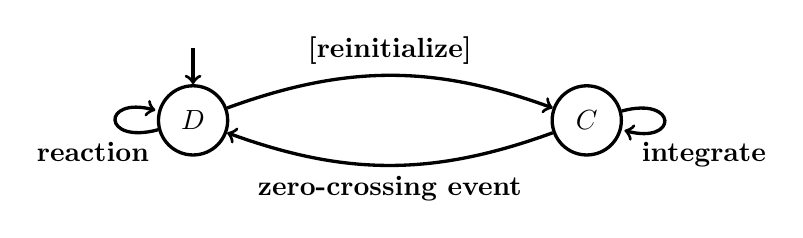
\begin{tikzpicture}[
      shift={(31.5,47.0)},
      ->,
      very thick,
      auto,
      node distance=5.0cm,
      initial where=above,
      font=\bfseries,
      initial text=]

     \node[state,initial] (D)		 {$D$};
     \node[state]         (C) [right of=D] {$C$};

     \path
       (D) edge [loop left] node[below left=.4em and -1.6em] {reaction} (D)
           edge [bend left=20]  node {[reinitialize]} (C)
       (C) edge [bend left=20]  node {zero-crossing event}    (D)
           edge [loop right] node[below right=.4em and -1.2em] {integrate}
           (C)
       ;

  \end{tikzpicture}
\end{center}

\begin{itemize}
\item Integration step (C):
\[
(y, z, t, h)(n+1) = 
                 \Solve{f_{\sigma(n)}}{g_{\sigma(n)}}((t, h, y)(n))
\quad \sigma(n+1) = \sigma(n)
\]
\item Discrete step (D):
\[
\begin{array}{l}
 (y, z, \sigma)(n+1) = d_{\sigma(n)}((z, t, y)(n)) \quad \quad
 t(n+1) = t(n) \\[2ex]
 h(n+1) = \Ifthenelse{t(n) = h(n)}{h(n)+step}{h(n)}
\end{array}
\]
\item From (D) to (C) when $\Not{z(n+1)}(i)$; $C$ to $D$ when $z(n+1)(i)$
\end{itemize}

%HEVEA\cutend

\chapter{Complete Examples}
\label{chapter:complete-examples}
%HEVEA\cutdef[1]{section}

We end this tutorial introduction with some typical examples. The
first one is the {\em inverted pendulum} which can be programmed in a
purely data-flow style. The second one is a simple controller for a
personal gas heater and illustrate the combination of data-flow
equations and state machines.  The next one is a simple version of the
coffee machine as defined by Milner in~\cite{milner:ccs-book89} and
adapted from Kevin Hammond description written in Hume~\cite{hume06}.
These examples show the compilation
and communication with the host language~\footnote{The full source
code of the examples is available in the distribution.}.

Other examples are available in the distribution of the language.

\section{The Inverted Pendulum}
Consider the problem of balancing an inverted pendulum with the hand
(through a mouse). The inverted pendulum has a length $l$, its bottom has 
coordinates $x_0$ and $y_0$ which are continuously controlled by the
user and it forms an angle $\theta$ with the
vertical. This pendulum is submitted to the following law:
\[
\begin{array}{ll}
\begin{array}{l}
  \mbox{\tt l} \times \frac{d^2\theta}{dt^2} \;=\; 
  (sin(\theta) \times (\frac{d^2\mbox{\tt y0}}{dt^2} + g)) - 
  (cos(\theta) \times \frac{d^2\mbox{\tt x0}}{dt^2})
\\
\mbox{\tt x} = \mbox{\tt x0} + \mbox{\tt l} \times sin(\theta)
\\
\mbox{\tt y} = \mbox{\tt y0} + \mbox{\tt l} \times cos(\theta)
\end{array}
&
\begin{array}{l}
%BEGIN IMAGE
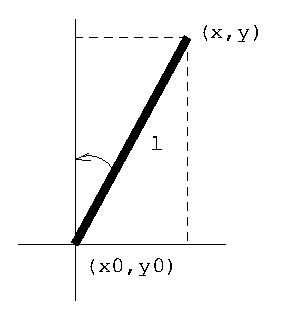
\includegraphics{Fig/pendulum}
%END IMAGE
%HEVEA \imageflush
\end{array}
\end{array}
\]

We suppose that some auxiliary scalar functions have been defined
in a \ocaml\ module \verb-Draw- with implementation \verb-draw.ml- and
interface \verb-draw.mli-. A pendulum is characterized by its
bottom and top coordinates. The exported values are defined below:

\begin{verbatim}
  (* file draw.mli *)
  type pendulum
  val make_pend : float -> float -> float -> float -> pendulum
  val clear_pend : pendulum -> unit
  val draw_pend : pendulum -> unit
  val mouse_pos : unit -> float * float
\end{verbatim}

\noindent
We start by defining a synchronous module for integrating and deriving
a signal.

\begin{verbatim}
  (* file misc.zls *)
  (* rectangle integration *)
  let node integr (t, x') = let rec x = 0.0 -> t *. x' +. pre x in x

  (* derivative *)
  let node deriv (t, x) = 0.0 -> (x -. (pre x))/. t
\end{verbatim}

\noindent Now, the main module defines global constants and the
pendulum law.

\begin{verbatim}
  (* file pendulum.zls *)
  open Draw
  open Misc

  let static t = 0.05 (* sampling frequency *)
  let static l = 10.0 (* length of the pendulum *)
  let static g = 9.81 (* acceleration *)

  let node integr x' = Misc.integr (t, x')
  let node deriv x = Misc.deriv (t, x)

  (* the equation of the pendulum *)
  let node equation (x0'', y0'') = theta
  where 
    rec theta =
        let thetap = 0.0 fby theta
        in integr (integr ((sin thetap) *. (y0'' +. g)
                          -.(cos thetap) *. x0'') /. l)

  let node position (x0, y0) = 
    let x0'' = deriv (deriv x0)  in
    let y0'' = deriv (deriv y0)  in

    let theta = equation (x0'', y0'') in

    let x = x0 +. l *. (sin theta)  in
    let y = y0 +. l *. (cos theta)  in
    make_pend x0 y0 x y
\end{verbatim}
As in \ocaml, an \verb-open- {\em Module} directive makes the names
exported by the module {\em Module} visible in the current
module~\footnote{The implemented module system of \zelus\ is borrowed
from \camllight, giving the minimal tools for importing names
from \ocaml\ files or from \zelus\ files.}. Imported values may be
either used with the dot notation (e.g, \verb-Draw.mouse_pos-) or
directly (e.g, \verb-make_pend-) once the module is opened.

Finally the main function continuously reads
informations from the mouse, computes the position of pendulum, clear
its previous position and draw its current position. We get:

\begin{verbatim}
  let node play () =
    let x0,y0 = mouse_pos () in
    let p = position (x0, y0) in
    clear_pendulum (p fby p);
    draw_pendulum p;;
\end{verbatim}

Now, all the files must be compiled. The compiler of \zelus\ acts as a
preprocessor: the compilation of the implementation \verb-misc.zls-
produces a file \verb-misc.ml- and a compiled interface
\verb-misc.lci- containing informations about types and clocks of the
implementation. Similarly, the compilation of the scalar interface
\verb-draw.mli- produces a compiled interface \verb-draw.lci-. Files
are compiled by typing:

\begin{verbatim}
  % zeluc draw.mli          => draw.lci
  % zeluc misc.zls          => misc.ml, misc.lci
  % zeluc pendulum.zls      => pendulum.ml
  % zeluc -s play -sampling 0.05 pendulum.lci
  
  % ocamlc draw.mli
  % ocamlc draw.ml
  % ocamlc pendulum.ml
  % ocamlc play.ml
  % ocamlc -o play draw.cmo pendulum.cmo play.cmo ...
\end{verbatim}
The whole system is obtained by linking all the modules
(synchronous and scalars ones) and by sampling the main transition 
function \verb-play- on a timer (here, 0.05 seconds) giving the base
clock (the real-time clock) of the system.

\section{The Heater}
\label{heater}
Consider the problem of a system which control a gas heater as
informally depicted in figure~\ref{figure-heater}.

\begin{figure}
\begin{center}
\begin{tabular}{cc}
%BEGIN IMAGE
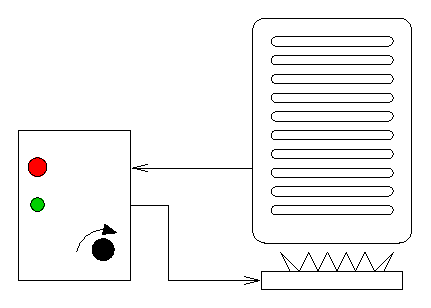
\includegraphics{Fig/heater}
%END IMAGE
&
%BEGIN IMAGE
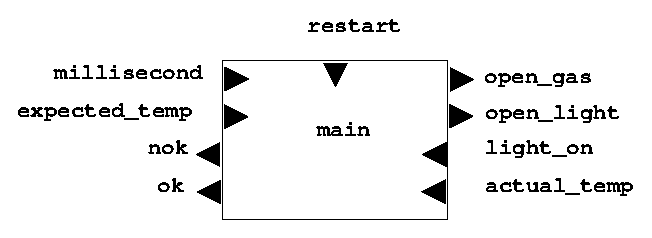
\includegraphics[width=0.5\textwidth]{Fig/heater_control}
%END IMAGE
%HEVEA\imageflush
\end{tabular}
\end{center}
\caption{The heater}\label{figure-heater}
\end{figure}

The heater front has a green light indicating a normal
functioning whereas the red light is turned on when some problem has
occurred (security stop). In that case, the heater is stopped and it can be restarted
by pushing a restart button.  Moreover, a rotating button allows the
user to indicate the expected temperature of the water.

The controller has thus the following inputs.
\begin{itemize}
\item
\verb-restart- is used to restart the heater.
\item
\verb-expected_temp- is the expected temperature of the water. The heater is
expected to maintain this temperature.
\item
\verb-actual_temp- is the actual temperature of the water measured by a
sensor.
\item
\verb-light_on- indicates that the light is on (that is, the gas is burning)
\item
\verb-millisecond- is a boolean flow given the clock of the system.
\end{itemize}
The outputs of the controller are the following:
\begin{itemize}
\item
\verb-open_light- opens the light command.
\item
\verb-open_gas- opens the valve for the gas.
\item
\verb-ok- indicate the status of the heater (controlling the green light)
whereas \verb-nok- indicates a problem (thus controlling the red light).
Only the \verb-restart- button can restart the heater.
\end{itemize}

The purpose of the controller is to keep the water temperature close
to the expected temperature. Moreover, when this temperature must be
heated, the controller turns on the gas and light for at most
\verb-500- millisecond. When the light is on, only the gas valve is
maintained open.  If there is no light after \verb-500- millisecond,
it stops for \verb-100- millisecond and start again. If after three
tests, there is still no light, the heater is blocked on a security
stop. Only pushing the \verb-restart- button allows to start again the
process.

We start with the definition of a few scalar constants and two auxiliary
functions.

\begin{verbatim}
let low = 4
let high = 4

let delay_on = 500 (* in miliseconds *)
let delay_off = 100

(* [count d t] returns [true] when [d] occurrences of [t] has been received *)
let node count (d, t) = ok where
  rec ok = cpt = 0
  and cpt = d -> if t & not (pre ok) then pre cpt - 1 else pre cpt

let node edge x = false -> not (pre x) & x
\end{verbatim}

The following node decides weather the heater must be turn on. We introduce
an hysteresis mechanism to avoid oscillation. \verb-low- and \verb-high- are
two threshold. The first version is a purely data-flow one whereas the
second one (which is equivalent) uses the automaton construction.

\begin{verbatim}
(* controling the heat *)
(* returns [true] when [expected_temp] does not agree with [actual_temp] *)
let node heat (expected_temp, actual_temp) = ok where
  rec ok = if actual_temp <= expected_temp - low then true
           else if actual_temp >= expected_temp + high then false
           else false -> pre ok

(* the same function using two modes *)
let node heat (expected_temp, actual_temp) = ok where
  rec automaton
      | False -> 
          do ok = false 
          unless (actual_temp <= expected_temp - low) then True
      | True ->
          do ok = true 
          unless (actual_temp >= expected_temp + high) then False
      end
\end{verbatim}

Now, we define a node which turns on the light and gas for 500 millisecond
then turn them off for 100 millisecond and restarts.

\begin{verbatim}
(* a cyclic two mode automaton with an internal timer *)
(* [open_light = true] and [open_gas = true] for [delay_on millisecond] *)
(* then [open_light = false] and [open_gas = false] for *)
(* [delay_off millisecond] *)
let node command millisecond = (open_light, open_gas) where
  rec automaton
      | Open ->
          do open_light = true
          and open_gas = true
          until (count delay_on millisecond) then Silent
      | Silent ->
          do open_light = false
          and open_gas = false
          until (count delay_off millisecond) then Open
      end
\end{verbatim}

The program which control the aperture of the light and
gas is written below:

\begin{verbatim}
(* the main command which control the opening of the light and gas *)
let node light (millisecond, on_heat, on_light) = 
    (open_light, open_gas, nok) where
  rec automaton
      | Light_off ->
          do nok = false
          and open_light = false
          and open_gas = false
          until on_heat then Try
      | Light_on ->
          do nok = false
          and open_light = false
          and open_gas = true
          until (not on_heat) then Light_off
      | Try ->
          do
            (open_light, open_gas) = command millisecond
          until light_on then Light_on
          until (count 3 (edge (not open_light))) then Failure
      | Failure ->
          do nok = true 
          and open_light = false
          and open_gas = false
          done
      end
\end{verbatim}

Finally, the main function connects the two parts.

\begin{verbatim}
(* the main function *)
let node main (millisecond, restart, expected_temp, actual_temp, on_light) =
                                       (open_light, open_gas, ok, nok) where
  rec reset
        on_heat = heat (expected_temp, actual_temp)
      and
        (open_light, open_gas,nok) = light (milisecond, on_heat, on_light)
      and
        ok = not nok       
      every restart
\end{verbatim}

Supposing that the program is written in a file \verb-heater.zls-, the
program can be compiled by typing:

\begin{verbatim}
% zeluc -s main heater.zls
\end{verbatim}
which produces files \verb-heater.ml- and \verb-main.ml-, the later
containing the transition function for the node \verb-main-.
 
\section{The Coffee Machine}
The following example is inspired from the Coffee Machine introduced
by Milner in his CCS book~\cite{milner:ccs-book89}.

The description is the following. The machine may serve coffee or tea.
A tea costs ten cents whereas a coffee costs five. The user may enter
dimes or nickels. He can select a tea, a coffee or ask for his money back.

\begin{verbatim}
type coin = Dime | Nickel
type drinks = Coffee | Tea
type buttons = BCoffee | BTea | BCancel


(* emits a drink if the accumulated value [v] is greater than [cost] *)
let node (vend, drink, cost, v) = (o1, o2) where
  match v >= cost with
  | true -> 
      do emit o1 = drink
      and o2 = v - cost
      done
  | false ->
      do o2 = v done
  end
\end{verbatim}
%
Now we define a function which output a drink and return some
money when necessary.
%
\begin{verbatim}
let node coffee (coin, button) = (drink, return) where
  rec last v = 0
  and present
      | coin(Nickel) -> 
          do v = last v + 5 done
      | coin(Dime) -> 
          do v = last v + 10 done
      | button(BCoffee) -> 
          do (drink, v) = vend Coffee 10 (last v)
          done
      | button(BTea) ->
          do (drink, v) = vend Tea 5 (last v)
          done
      | button(BCancel) ->
          do v = 0
          and emit return = last v
          done
      end
\end{verbatim}
%
The function \verb-coffee- can be also written like the following.
%
\begin{verbatim}
let node coffee (coin, button) = (drink, return) where
  rec init v = 0
  and present
      | coin(w) ->
          do match w with
               Nickel -> do v = last v + 5 done
             | Dime -> do v = last v + 10 done
             end
          done
      | button(b) ->
          do match b with
               BCoffee -> do (drink, v) = vend Coffee 10 (last v) done
             | BTea -> do (drink, v) = vend Tea 5 (last v) done
             | BCancel -> do v = 0 and emit return = last v done
             end
          done
       end
\end{verbatim}
We end by adding the code for simulating the whole system.

\begin{verbatim}
(* producing events from the keyboard *)
let node input key = (coin, button) where
  match key with
    "N" -> do emit coin = Nickel done
  | "D" -> do emit coin = Dime done
  | "C" -> do emit button = BCoffee done
  | "T" -> do emit button = BTea done
  | "A" -> do emit button = BCancel done
  | _ -> do done
  end

(* printing things *)
let print_drink d =
  match d with 
    Coffee -> print_string "Coffee\n"
  | Tea -> print_string "Tea\n"
  end

let print_coin d =
  match d with 
    Nickel -> print_string "Nickel\n"
  | Dime -> print_string "Dime\n"
  end

let print_button d =
  match d with 
    BCoffee -> print_string "BCoffee\n"
  | BTea -> print_string "BTea\n"
  | BCancel -> print_string "BCancel\n"
  end

let node output (drink, return) =
   present dringk(d) -> print_drink d;
   present return(r) -> print_int r

let node main () =
  let key = read_line () in
  let (coin, button) = input key in
  let drink, return = coffee (coin, button) in
  output (drink, return)
\end{verbatim}

The final application is obained by typing:

\begin{verbatim}
%zeluc -s main -sampling 0 coffee.zls
%ocamlc -o main coffee.ml main.ml
\end{verbatim}

\Marc{Ajouter un joli example hybride}
%HEVEA\cutend

\cleardoublepage

\part{Reference manual}
\label{reference-manual}
\cleardoublepage
\chapter{The language}

%HEVEA\cutdef[1]{section}

% Shamelessly stole from the OCaml manual
The syntax of the language is given in BNF-like notation. Terminal
symbols are set in typewriter font (\term{like this}). Non-terminal symbols
are set in italic font (\nterm{like that}). Square brackets [ ... ] denote
optional components. Curly brackets \{ ... \} denotes zero, one or several
repetitions of the enclosed components.

% We follow the following convention for grammatical rules. If $t$ is
% a syntactical entity, $\{\;t\;\}$ denotes the arbitrary repetition of $t$.

\section{Lexical conventions}

Lexical conventions for blanks, comments, identifiers, integer
literals, floating-point literals, character literals, string
literals, prefix and infix symbols are the one of \ocaml.

\subsubsection{Keywords}
The following identifiers are keywords.

\begin{verbatim}
      let  and   if    then  pre   or   node  done      unless   run   end
      rec  where fun   else  not   open match automaton continue emit
      fby  reset every do   until  on   der   init      hybrid
\end{verbatim}
The following character sequences are also keywords:

\begin{verbatim}
        ->   >     <     =     <>     >=        )     &  ?
        +    -     *     /     ;;     <=        (     .
\end{verbatim}

\section{Values}

\subsection{Basic values}
\zelus{} only implements the basic values of \ocaml{} with the same
convention, that is, integer numbers, floating-point numbers,
characters and character strings.
\subsection{Tuples, records, sum types}
\zelus{} implements the tuples of \ocaml, with the same conventions. It
also implements records and sum types.

\subsubsection{Functions and nodes}
Mapping from values to values. Functions are stateless mapping whereas
nodes denote possibly stateful values.

\section{Global names}
\label{global-names}
The naming conventions in \zelus{} are inherited from \ocaml, with some
restrictions. They are listed here:

Names in \zelus{} are decomposed into the following syntactic classes:
\begin{itemize}
\item
  The syntactic class \nterm{value-name} for value names
\item
  The syntactic class \nterm{typeconstr-name} for type constructors
\item
  The syntactic class \nterm{module-name} for module names
\end{itemize}

\subsection{Naming values}

\begin{center}
\begin{tabular}{lcl}
\nterm{value-name}       & ::=    & \nterm{lowercase-ident} \\
                         & $\;\;\alt$ & \term{(} \nterm{operator-name}
                                        \term{)} \\
\nterm{operator-name}    & ::=    & \nterm{prefix-symbol} 
                           $\alt$   \nterm{infix-symbol} 
                           $\alt$   \term{*} $\alt$ \term{=} $\alt$ \term{or}
                           $\alt$   \term{\&} \\
\nterm{constructor-name} & ::=    & \nterm{capitalized-ident} \\
                         & $\;\;\alt$ & \term{()} \\
\nterm{typeconstr-name}  & ::=    & \nterm{lowercase-ident} \\
\nterm{module-name}      & ::=    & \nterm{capitalized-ident}
\end{tabular}
\end{center}

The syntactic class of \nterm{lowercase-ident} is the
set of identifiers starting with a lowercase letter whereas
\nterm{capitalized-ident} is the set of of identifiers starting with a
capital letter.

\subsection{Referring to named values}
\begin{center}
\begin{tabular}{lcl}
\nterm{value-path}  & ::=        & \nterm{value-name} \\
                    & $\;\;\alt$ & \nterm{module-name} \term{.}
                                   \nterm{value-name} \\
\nterm{constructor} & ::=        & \nterm{constructor-name} \\
                    & $\;\;\alt$ & \nterm{module-name} \term{.}
                                   \nterm{capitalized-ident} \\
\nterm{typeconstr}  & ::=        & \nterm{typeconstr-name} \\
                    & $\;\;\alt$ & \nterm{module-name} \term{.} 
                                   \nterm{typeconstr}
\end{tabular}
\end{center}
A value can be referred either by its name or by qualifying the name
with a module name.

\section{Types}
\begin{center}
\begin{tabular}{lcl}
\nterm{type} & ::=        & \term{'} \nterm{ident} \\
             & $\;\;\alt$ & \term{(} \nterm{type} \term{)} \\
             & $\;\;\alt$ & \nterm{type} \term{->} \nterm{type} \\
             & $\;\;\alt$ & \nterm{type} \{\term{*} \nterm{type}\} \\
             & $\;\;\alt$ & \nterm{type} \nterm{typeconstr} \\
             & $\;\;\alt$ & \term{(} \nterm{type} \{\term{,}
                            \nterm{type} \}\term{)} \nterm{typeconstr} \\
             & $\;\;\alt$ & \nterm{typeconstr}
\end{tabular}
\end{center}

The precedences are given in the following table. The constructions
with higher precedences come first.
\begin{center}
\begin{tabular}{|l|l|}
\hline
Operator                        & Associativity \\ \hline
{\tt sig}                       & -            \\ 
{\tt *}                         & -             \\
{\tt ->}                        & right         \\ \hline
\end{tabular}
\end{center}

\section{Constants}

\begin{center}
\begin{tabular}{lcl}
\nterm{immediate} & ::=           & \nterm{integer-literal} \\
                  & $\;\;\alt$    & \nterm{float-literal} \\
                  & $\;\;\alt$    & \nterm{char-literal} \\
                  & $\;\;\alt$    & \nterm{string-literal} \\
                  & $\;\;\alt$    & \nterm{boolean-literal} \\
\end{tabular}
\end{center}
Constants are made of literals from the firth base types (integers,
floating-point numbers, characters, character strings and booleans).

\section{Patterns}
\begin{center}
\begin{tabular}{lcl}
\nterm{pattern} & ::=        & \nterm{ident} \\
                & $\;\;\alt$ & \term{(} \nterm{pattern} \term{)} \\
                & $\;\;\alt$ & \nterm{pattern} \term{as} \nterm{ident} \\
                & $\;\;\alt$ & \term{\_} \\
                & $\;\;\alt$ & \nterm{pattern} \term{,} \nterm{pattern} 
                               \{ \term{,} \nterm{pattern} \} \\
                & $\;\;\alt$ & \term{()} \\
                & $\;\;\alt$ & \nterm{immediate} \\
                & $\;\;\alt$ & \nterm{constructor} \\
                & $\;\;\alt$ & \nterm{constructor} \nterm{pattern} \\
                & $\;\;\alt$ & \term{\{} \nterm{label} 
                               \term{=} \nterm{pattern} \{ \term{;} 
                               \nterm{label} \term{=} \nterm{pattern}
                               \} \term{\}} \\
%       & $\alt$ & pattern \mbox{\tt when} ident \\
                & $\;\;\alt$ & \nterm{clock} \nterm{ident} \\
                & $\;\;\alt$ & \term{static} \nterm{ident}
\end{tabular}
\end{center}
Patterns allow selecting data structures of a given shape and binding
identifiers to components of the data structure.

\section{Signal Patterns}
\begin{center}
\begin{tabular}{lcl}
\nterm{signal-pattern} 
   & ::=        & \nterm{simple-expr} \\
   & $\;\;\alt$ & \nterm{simple-expression} \nterm{pattern} \\ 
   & $\;\;\alt$ & \nterm{signal-pattern} \term{\&} \nterm{signal-pattern}
\end{tabular}
\end{center}
Signal patterns allows to test the presence of signals and to match
their value with some pattern. Moreover, a signal pattern can be also
a boolean expression.

\section{Expressions}
\label{expressions}
\begin{center}
\begin{tabular}{lcl}
\nterm{simple-expr}
  & ::=        & \nterm{value-path} \\
  & $\;\;\alt$ & \nterm{constructor} \\
  & $\;\;\alt$ & \nterm{constructor} \nterm{expr} \\
  & $\;\;\alt$ & \nterm{immediate} \\
  & $\;\;\alt$ & \term{(} \nterm{expr} \term{)} \\
  & $\;\;\alt$ & \term{\{} \nterm{label} \term{=} \nterm{expr}
                 \{ \term{;} \nterm{label} \term{=} \nterm{expr} \} 
                 \term{\}} \\
  & $\;\;\alt$ & \nterm{simple-expr} \term{.} \nterm{label}
\\ \\
\nterm{multiple-matching}
   & ::=        & \nterm{pattern-list} \term{\Minusgreater} \nterm{expr} \\
   & $\;\;\alt$ & \nterm{pattern-list} \term{\Equalgreater} \nterm{expr} 
\\ \\
\nterm{pattern-list}           
   & ::=        & \nterm{pattern} \{ \nterm{pattern} \}
\end{tabular}
\end{center}

\begin{center}
\begin{tabular}{lcl}
\nterm{expr}
   & ::=        & \nterm{simple-expr} \\
   & $\;\;\alt$ & \nterm{simple-expr} \nterm{simple-expr} \{ \nterm{simple-expr} \} \\
   & $\;\;\alt$ & \term{\Fun} \nterm{multiple-matching} \\
%                       & $\alt$ & \Function\ simple-matching \\
   & $\;\;\alt$ & \nterm{simple-expr} \term{\Where} [ \term{\Rec} ]
                  \nterm{definition} \{ \term{\And} \nterm{definition}
                  \} \\
   & $\;\;\alt$ & \term{\Let} [ \term{\Rec} ] \nterm{definition}
                  \{ \term{\And} \nterm{definition} \} \term{\In} 
                  \nterm{expr} \\
   & $\;\;\alt$ & \term{\If} \nterm{expr} \term{\Then} \nterm{expr}
                  \term{\Else} \nterm{expr} \\
%                       & $\alt$ & \Match{expr}{pattern-matching} \\
   & $\;\;\alt$ & \nterm{prefix-op} \nterm{expr} \\
   & $\;\;\alt$ & \nterm{expr} \nterm{infix-op} \nterm{expr} \\
   & $\;\;\alt$ & \nterm{expr} \term{\Or} \nterm{expr} \\
   & $\;\;\alt$ & \term{\Not} \nterm{expr} \\
      & $\;\;\alt$ & \nterm{expr} \term{\Fby} \nterm{expr} \\
   & $\;\;\alt$ & \term{\Pre} \nterm{expr} \\
   & $\;\;\alt$ & \term{\Last} \nterm{ident} \\
   & $\;\;\alt$ & \nterm{expr} \term{\Minusgreater} \nterm{expr} \\
   & $\;\;\alt$ & \term{\Run} \nterm{simple-expr} \{ \nterm{simple-expr} \} \\
   & $\;\;\alt$ & \term{match} \nterm{expr} \term{with} 
                  \nterm{match-handlers} \term{end} \\
   & $\;\;\alt$ & \term{reset} \nterm{expr} \term{every} \nterm{expr} \\ 
   & $\;\;\alt$ & \term{present} \nterm{present-handlers} \term{end}
%                       & $\alt$ & \Reset\ expr expr \{ expr\} \Every\ expr
\\
\\
\nterm{match-handlers}
   & ::=        & [ \term{|} ] 
                  \nterm{pattern} \term{\Minusgreater} \nterm{expr}
                  \{ \term{|} 
                  \nterm{pattern} \term{\Minusgreater} \nterm{expr} \}
\\
\\
\nterm{present-handlers}
   & ::=        & [ \term{|} ] 
                  \nterm{signal-pattern} \term{->} \nterm{expr}
                  \{ \term{|}
                  \nterm{signal-pattern} \term{->} \nterm{expr} \} 
\end{tabular}
\end{center}

The precedence and associativity rules are the one of \ocaml. For
special \zelus\ primitives, they are given below:
higher precedences come first.
\begin{center}
{
\begin{tabular}{|l|l|} \hline
\Last                           & right         \\
\Pre                            & -             \\
function application            & right         \\
\Fby                            & left          \\
...
\Let,...                        & -             \\ 
\Minusgreater                   & right         \\ \hline
\end{tabular}
}
\end{center}

\subsection{Simple expressions}

\subsubsection{Constants}
Expressions consisting in a constant evaluate to an infinite stream
made of this constant.

\subsubsection{Variables}
Expressions consisting in a variable evaluate to the value bound to
this variable in the current evaluation environment.

\subsubsection{Parenthetised expressions}
The expression \term{(} \nterm{expr} \term{)} has the same value than
\nterm{expr}.

\subsubsection{Function abstraction}
A function abstraction has two forms: 
\begin{center}
\begin{tabular}{l}
\term{fun} \nterm{pattern}$_1$ ... \nterm{pattern}$_n$ \term{->} \nterm{expr}
\end{tabular}
\end{center}
defines a {\em combinatorial} (or state-less) function. This means
that expression \nterm{expr} must not contain any state constructions.
\begin{center}
\begin{tabular}{l}
\term{fun} \nterm{pattern}$_1$ ... \nterm{pattern}$_n$ \term{=>} \nterm{expr}
\end{tabular}
\end{center}
defines a {\em sequential} (or state-full) function.

\subsubsection{Function application}
The expression \nterm{expr}$_1$ \nterm{expr}$_2$ is an
application. The expression \nterm{expr}$_1$ must evaluate to a
functional value which is applied to the value of \nterm{expr}$_2$.

The expression \nterm{expr}$_1$ \nterm{expr}$_2$ ... \nterm{expr}$_n$
stands for (...(\nterm{expr}$_1$ \nterm{expr}$_2$) ...
\nterm{expr}$_n$). No evaluation order is specified.

When \nterm{expr}$_1$ is a function imported from the host language
\ocaml\ and \nterm{expr}$_2$ is a stream then \nterm{expr}$_1$
\nterm{expr}$_2$ stands for the point-wise application of
\nterm{expr}$_1$ to every element of \nterm{expr}$_2$.

\subsubsection{Local definitions}
The \term{\Let} and \term{\Let\ \Rec} constructs bind variables
locally. The expression 
\begin{center}
  \term{\Let} \nterm{definition}$_1$ \term{\And} ... 
  \term{\And} \nterm{definition}$_n$ \term{\In} \nterm{expr}
\end{center}
defines values to be visible in \nterm{expr}.

Recursive definitions of variables are introduced by \term{\Let\ \Rec}:
\begin{center}
  \term{\Let\ \Rec} \nterm{definition}$_1$ \term{\And} ... 
  \term{\And} \nterm{definition}$_n$ \term{\In} \nterm{expr}
\end{center}

\subsubsection{Reverse local definition}
The language provides an alternate form of local definitions written
in a reverse order and borrowed from \camllight.  In this way,
functions may be defined is a way similar to \lustre. The expression:
\begin{center}
  \nterm{simple-expr} \term{\Where} [ \term{\Rec} ] 
  \nterm{definition}$_1$ \term{\And} ... \term{\And} \nterm{definition}$_n$
\end{center}
has the meaning of:
\begin{center}
  \term{\Let} [ \term{\Rec} ] 
  \nterm{definition}$_1$ \term{\And} ... \term{\And} \nterm{definition}$_n$
  \term{\In} \nterm{expr}
\end{center}

\subsection{Operators}
The operators written \nterm{infix-op} in the grammar can appear in
infix position (between two expressions). The operators written
\nterm{prefix-op} in the grammar (section~\ref{expressions} can appear
in prefix position (in front of an expression).

Classical operators provided by \ocaml\ (from the {\tt Pervasives}
module) are imported. As for general scalar value imported from the
host language, they become stream operators which are applied
point-wisely to streams.

\subsubsection{Delays}
The expression \term{\Pre} \nterm{expr} is the delayed
stream. \nterm{expr} must be a stream. The clock of the result is the
clock of \nterm{expr}. The $n$-th value of the result is the $n-1$-th
value of \nterm{expr}. Its value at the first instant is undefined.

The binary operator \term{\Fby} is the initialized delay operator. The
first value of \nterm{expr}$_1$ \term{\Fby} \nterm{expr}$_2$ is the
first value of \nterm{expr}$_1$. Its $n$-th value is the $n-1$-th
value of \nterm{expr}$_2$.

\subsubsection{Shared Memory}
The expression \term{\Last} \nterm{ident} denotes a shared memory
which contains the last computed value of \nterm{ident}.

\subsubsection{Initialization}
\nterm{expr}$_1$ \term{\Minusgreater} \nterm{expr}$_2$ initializes a
stream. The \nterm{expr}$_i$ must be streams of the same type and on
the same clock. It returns a stream with the same type and clock. The
first value of the result is the first value of
\nterm{expr}$_1$. Then, the $n$-th value of the result is the $n$-th
value of \nterm{expr}$_2$.

\subsubsection{Point-wise conditional}
The expression \term{\If} \nterm{expr}$_1$ \term{\Then}
\nterm{expr}$_2$ \term{\Else} \nterm{expr}$_3$ is the point-wise
conditional. \nterm{expr}$_1$ must be a boolean stream,
\nterm{expr}$_2$ and \nterm{expr}$_3$ two streams of the same
type. The type of the result is the type of \nterm{expr}$_2$. The
expressions \nterm{expr}$_i$ must be on the same clock. The clock of
the result is the clock of \nterm{expr}$_1$. The conditional returns a
stream such that its $n$-th value is the $n$-th value of
\nterm{expr}$_2$ if the $n$-th value of \nterm{expr}$_1$ is true and
the $n$-th value of \nterm{expr}$_3$ otherwise.

\subsection{Control Structures}
The constructions \verb-reset-, \verb-match/with-, \verb-reset- and
\verb-automaton- are control-structures which combine equations and
thus belong to the syntactic class of definitions (see
section~\ref{definitions}).

A derived form belonging to the syntactic class of expressions is also
provided. The derived form is useful for textual programming whereas
the original one is motivated by the graphical representation of
dataflow programs. The derived form is only syntactic sugar for the
original form.

\subsubsection{Pattern Matching}
The expression
\term{match} \nterm{expr} \term{with} 
  \nterm{pat}$_1$ \term{\Minusgreater} \nterm{expr}$_1$ \term{|} \dots 
\term{|} \nterm{pat}$_n$ \term{\Minusgreater} \nterm{expr}$_n$ \term{end}
is a short-cut for the expression:

\begin{center}
\begin{tabbing}
\term{let} \= \term{match} \nterm{expr} \term{with} \\ 
           \> \term{|} \nterm{pat}$_1$ \term{\Minusgreater} 
               \term{do} \nterm{o} \term{=} \nterm{expr}$_1$ \term{done} \\
           \> \dots \\
           \> \term{|} \nterm{pat}$_n$ \term{\Minusgreater} 
               \term{do} \nterm{o} \term{=} \nterm{expr}$_n$ \term{done} \\
           \> \term{end} \In \\
\nterm{o}
\end{tabbing}
\end{center}
provided \nterm{o} is a fresh name.

\subsubsection{Modular Reset}
The expression \term{reset} \nterm{expr}$_1$ \term{every} \nterm{expr}$_2$
is a short-cut for
\term{let reset} \nterm{o} \term{=} \nterm{expr}$_1$ 
\term{every} \nterm{expr}$_2$ \term{in} \nterm{o},
provided \nterm{o} is a fresh name.

\subsubsection{Automata}
The expression 
\term{automaton} \nterm{state}$_1$ \term{\Minusgreater} \nterm{expr}$_1$ 
                 \nterm{trans}$_1$ 
\term{|} \dots
\term{|} \nterm{state}$_n$ \term{\Minusgreater} \nterm{expr}$_n$ 
                 \nterm{trans}$_n$ \term{end} is a short-cut
for the expression:

\begin{tabbing}
let \= \term{automaton} \\
    \> \term{|} \nterm{state}$_1$ \term{\Minusgreater} 
                 \term{do} \nterm{o} = \nterm{expr}$_1$ \nterm{trans}$_1$ \\
    \> \dots \\
    \> \term{|} \nterm{state}$_n$ \term{\Minusgreater} 
              \term{do} \nterm{o} = \nterm{expr}$_n$ \nterm{trans}$_n$ \\
    \> \term{end in} \\
\nterm{o}
\end{tabbing}
provided \nterm{o} is a fresh name.

\subsubsection{Testing the Presence}
The expression
\term{present}
  \nterm{spat}$_1$ \term{\Minusgreater} \nterm{expr}$_1$ \term{|} \dots 
\term{|} \nterm{spat}$_n$ \term{\Minusgreater} \nterm{expr}$_n$ \term{end}
is a short-cut for the expression:

\begin{center}
\begin{tabbing}
\term{let} \= \term{present} \\
           \> \term{|} \nterm{spat}$_1$ \term{\Minusgreater} 
               \term{do} \nterm{o} \term{=} \nterm{expr}$_1$ \term{done} \\
           \> \dots \\
           \> \term{|} \nterm{spat}$_n$ \term{\Minusgreater} 
               \term{do} \nterm{o} \term{=} \nterm{expr}$_n$ \term{done} \\
           \> \term{end} \In \\
\nterm{o}
\end{tabbing}
\end{center}
provided \nterm{o} is a fresh name.

\section{Definitions}
\label{definitions}
\begin{center}
\begin{tabular}{lcl}
\nterm{let-binding}
   & ::=        & \nterm{pattern} \term{=} \nterm{expr} \\
   & $\;\;\alt$ & \nterm{ident} \nterm{pattern-list} \term{=} \nterm{expr} \\
   & $\;\;\alt$ & \term{node} \nterm{ident} \nterm{pattern-list} 
                  \term{=} \nterm{expr} \\
   & $\;\;\alt$ & \term{last} \nterm{ident} \term{=} \nterm{expr} \\
   & $\;\;\alt$ & \term{emit} \nterm{ident} \term{=} \nterm{expr}
%                       & $\alt$ & {\tt clock} ident {\tt =} expr \\
\\ \\
\nterm{infix-op}                
   & ::=        & \nterm{infix-symbol} 
                  $\alt$ \term{*} 
                  $\alt$ \term{=} 
                  $\alt$ \term{or}  
                  $\alt$ \term{\&}
\\ \\
\nterm{definition} 
   & ::=        & \nterm{let-binding} \\
   & $\;\;\alt$ & \term{match} \nterm{expr} \term{with}  
                  \nterm{def-match-handlers} \term{end} \\
   & $\;\;\alt$ & \term{\Reset} \nterm{definition} 
                  \{ \term{\And} \nterm{definition} \}
                  \term{\Every} \nterm{expr} \\
   & $\;\;\alt$ & \term{automaton} \nterm{def-automaton-handlers}
                  \term{end} \\
   & $\;\;\alt$ & \term{present} \nterm{def-present-handlers} \term{end}
\\ \\
\nterm{definition-list}
   & ::=        & [ \nterm{definition} \{ \term{\And}
                  \nterm{definition} \} ] \\ 
   & $\;\;\alt$ & $\epsilon$
\\ \\
\nterm{local-definitions}      
   & ::=        & \{ \term{\Let} [ \term{\Rec} ] \nterm{definition}
                  \{ \term{\And} \nterm{definition} \} \term{\In} \}
\\ \\
\nterm{def-match-handlers}
   & ::=        & [ \term{|} ] \nterm{def-match-handler}
                  \{ \term{|} \nterm{def-match-handler} \} 
\\ \\
\nterm{def-match-handler}
   & ::=        & \nterm{pattern} \term{\Minusgreater} \nterm{action}
\\ \\
\nterm{action}                  
   & ::=        & \nterm{local-definitions}
                  \term{\Do} \nterm{definition-list} \term{\Done}
\\ \\
\nterm{def-automaton-handlers}
   & ::=        & [ \term{|} ] \nterm{def-automaton-handler}
                  \{ \term{|} \nterm{def-automaton-handler} \} 
\\ \\
\nterm{def-automaton-handler}
   & ::=        & \nterm{constructor} [ \nterm{pattern} ] \term{->}
                  \nterm{automaton-action}
\\ \\
\nterm{automaton-action}
   & ::=        & \nterm{local-definitions}
                  \term{\Do} \nterm{definition-list} \nterm{def-transitions}
\\ \\
\nterm{def-transitions}
   & ::=        & \term{\Done} \\
   & $\;\;\alt$ & \term{\Then} \nterm{state-expression} \\
   & $\;\;\alt$ & \term{\Continue} \nterm{state-expression} \\
   & $\;\;\alt$ & \nterm{transition} \{ \nterm{transition} \}
\\ \\
\nterm{state-expression}
   & ::=        & \nterm{constructor} \\
   & $\;\;\alt$ & \nterm{constructor} \term{(} \nterm{expr} \term{)}
\\ \\
\nterm{def-present-handlers}
   & ::=        & [ \term{|} ] \nterm{def-present-handler}
                  \{ \term{|} \nterm{def-present-handler} \} 
\\
\nterm{def-present-handler}
   & ::=        & \nterm{signal-pattern} \term{->} 
                  \nterm{action} \term{\Done} \\
   & $\;\;\alt$ & \term{\_} \term{->} \nterm{action} \term{\Done}
\end{tabular}
\end{center}

\subsubsection{Value Definition}
A definition \nterm{pattern} \term{=} \nterm{expr} defines variables
and is obtained by matching the value of \nterm{expr} with
\nterm{pattern}. An alternate syntax is provided to define functional
values. The definition:
\begin{center}
  \nterm{ident} \term{=} \term{\Fun} \nterm{pattern}$_1$ ...
  \nterm{pattern}$_n$ \term{\Arrow} \nterm{expr}
\end{center}
can be declared in the following way:
\begin{center}
  \nterm{ident} \nterm{pattern}$_1$ ... \nterm{pattern}$_n$ 
  \term{=} \nterm{expr}
\end{center}
And the definition:
\begin{center}
  \nterm{ident} \term{=} \term{\Fun}
  \nterm{pattern}$_1$ ... \nterm{pattern}$_n$ \term{=>} \nterm{expr}
\end{center}
can be declared in the following way:
\begin{center}
  \term{\Node} \nterm{ident} \nterm{pattern}$_1$ ...
  \nterm{pattern}$_n$ \term{=} \nterm{expr}
\end{center}
Both forms define \nterm{ident} to be a function with $n$ arguments.

\subsubsection{Shared Memory Initialization}
A definition \term{\Last} \nterm{ident} \term{=} \nterm{expr} defines
a shared memory \term{\Last} \nterm{ident} to be initialized with the
value of \nterm{expr}.

\subsubsection{Signal Definition}
A definition \term{\Emit} \nterm{ident} \term{=} \nterm{expr} defines
the signal \nterm{ident} to be equal to the value of \nterm{expr}.

\subsubsection{Pattern Matching}
\term{match} \nterm{expr} \nterm{pattern}$_1$ \term{->}
\nterm{action}$_1$ \term{|} ... \term{|} \nterm{pattern}$_n$ \term{->}
\nterm{action}$_n$ \term{end} is used for combining $n$ complementary
sub-streams. Each of these streams is on the clock defined by the
instants where the value of $e$ has the form \nterm{pattern}$_i$\ .

Each \nterm{action} is made of a (possibly empty) sequence of local
definitions and a definition list of shared variables. These shared
variables can appear in several branches.

\subsubsection{Modular Reset}
The construction \term{\Reset} \nterm{definition}$_1$ \term{\And} ...
\term{\And} \nterm{definition}$_n$ \term{\Every} \nterm{expr} allows
for resetting the computation made in a set of definitions. All the
defined values and expression \nterm{expr} must be on the same
clock. This construction acts as a regular multi-definition except
that all the streams and automata defined in
\nterm{definition}$_1$,..., \nterm{definition}$_n$ restart with their
initial value every time the current value of {\em expr} is true. In
particular automata restart into their initial state.

\subsubsection{Automata}
The construction \term{automaton} \nterm{def-automaton-handler} \term{|}
... \term{|} \nterm{def-automaton-handler} \term{end} defines an
automaton. Each branch of the automaton is of the form:
\begin{center} 
  \nterm{constructor} \term{->} \nterm{automaton-action}
\end{center}
or
\begin{center}
  \nterm{constructor} \nterm{pattern} \term{->} \nterm{automaton-action}
\end{center}
where \nterm{constructor} denotes the name of the state. This state
may be parameterized by a pattern.  The first branch defines the
initial state and this state cannot be parameterized.

The action associated to a state is of the form:
\begin{center}
  \nterm{local-definitions} \term{\Do} \nterm{definition-list} 
  \nterm{transitions}
\end{center}
It is made of a (possibly empty) sequence of local definitions to the
state, a definition list of shared variables and a (possibly empty)
list of transitions which are tested sequentially. Transitions may
have several forms.  Writing:
\begin{center}
  \term{\Until} \nterm{signal-pattern} \term{\Then} \nterm{state-expression}
\end{center}
defines a {\em weak transition} which is executed at the end of the
reaction, that is, {\em after} definitions from the current state have
been executed. When the conditions succeed, the new state is given by
the value of \nterm{state-expression}. The keyword \term{\Then}
indicates that the new state is {\em entered by reset}, that is, all
the streams and automata in the next state restart with their initial
value.  Writing: \begin{center} \term{\Until} \nterm{signal-pattern} 
\term{\Continue} \nterm{state-expression}
\end{center}
has the same behavior except that the next state is {\em entered by
  history}, that is, no reset occurs.

The language provides two derived forms of transitions written
\term{\Then} \nterm{state-expression} and \term{\Continue}
\nterm{state-expression} as short-cut of \term{\Until} {\tt true}
\term{\Then} \nterm{state-expression} and \term{\Until} {\tt true}
\term{\Continue} \nterm{state-expression}.

Moreover, transitions may be either weak of strong. The following form:
\begin{center}
  \term{\Unless} \nterm{signal-pattern} \term{\Then} \nterm{state-expression}
\end{center}
defines a {\em strong transition} which is executed {\em before} the
reaction starts, that is, before definitions from the current state
have been executed. When the conditions succeed, the definitions to be
executed belong to the value of \nterm{state-expression}. The keyword
\term{\Then} indicates that the new state is entered by reset, that is,
every stream and state from the value of \nterm{state-expression} are
reseted. Finally, writing: \begin{center}
  \term{\Unless} \nterm{signal-pattern} \term{\Then} \nterm{state-expression}
\end{center}
defines a strong transition with entrance by history.

\subsubsection{Testing the Presence of Signals}
A present statement is pretty much the same as a pattern-matching
statement. It is of the form: 
\begin{center}
  \term{present} \nterm{def-present-handler}$_1$ 
  \term{|} ... \term{|} \nterm{def-present-handler}$_n$ \term{end}
\end{center}
Where a handler is of the form:
\begin{center}
  \nterm{signal-pattern} \term{->} \nterm{action}
\end{center}
Signal patterns are tested sequentially and the one which succeed
defines the corresponding action to execute. Finally, a handler:
\begin{center} 
  \term{\_} \term{->} \nterm{action}
\end{center}
defines a condition which always succeed.

\section{Type definition}
Abstract types can be defined. Their syntax is inherited from \ocaml\
and is reminded here. 
\begin{center}
\begin{tabular}{lcl}
\nterm{type-definition} 
  & ::=    & \term{type} \nterm{typedef} 
             \{ \term{and} \nterm{typedef} \} 
\\ \\
\nterm{typedef}
  & ::=        & [ \nterm{type-params} ] \nterm{typeconstr-name} \\
  & $\;\;\alt$ & \nterm{sum-type-def} \\
  & $\;\;\alt$ & \nterm{record-type-def} 
\\ \\
\nterm{sum-type-def}
  & ::=        & [ \term{|} ] \nterm{one-sum-def} 
                 \{ \term{|} \nterm{one-sum-def} \} 
\\ \\
\nterm{one-sum-def}     
  & ::=        & \nterm{capitalized-ident} \\
  & $\;\;\alt$ & \nterm{capitalized-ident} \term{of} \nterm{type} 
\\ \\
\nterm{record-type-def} 
  & ::=        & \term{\{} \nterm{label-type}
                 \{ \term{;} \nterm{label-type} \} \term{\}} 
\\ \\
\nterm{label-type}
  & ::=        & \nterm{ident} \term{:} \nterm{type} 
\\ \\
\nterm{type-params}
  & ::=        & \term{'} \nterm{ident} \\
  & $\;\;\alt$ & \term{(} \term{'} \nterm{ident} 
                 \{ \term{,} \term{'} \nterm{ident} \} \term{)}
\end{tabular}
\end{center}

\section{Module implementation}
\begin{center}
\begin{tabular}{lcl}
\nterm{implementation}
  & ::=        & \{ \nterm{impl-phrase} [ \term{;;} ] \} 
\\ \\
\nterm{impl-phrase}
  & ::=        & \nterm{value-definition} \\ 
  & $\;\;\alt$ & \nterm{type-definition} \\
  & $\;\;\alt$ & \term{open} \nterm{module-name} 
\\ \\
\nterm{value-definition} 
  & ::=        & \term{\Let} [ \Rec ]
                 \nterm{let-binding} 
                 \{ \term{\And} \nterm{let-binding} \}
                 [ \term{;} ]
\end{tabular}
\end{center}
A module implementation consists in a sequence of implementation
phrases. An implementation phrase either opens a module, is a type
definition or is a sequence of definitions.
\begin{itemize}
\item The instruction \term{open} modifies the list of opened modules
  by adding the module name to the list of opened modules, in first
  position.
\item The type definition defines the type for the implementation
  phrases following the definition.
\item The value definition defines some global values.
\end{itemize}

\section{Scalar Interfaces and Importing values}
Scalar interfaces written in \ocaml\ can be imported by \zelus. In the
current implementation, a restricted subset of \ocaml\ interfaces is
considered. The syntax is the following:
\begin{center}
\begin{tabular}{lcl}
\nterm{scalar-interface}
  & :: =   & \{ \nterm{scalar-interface-phrase} [ \term{\Semisemi} ] \} 
\\ \\
\nterm{scalar-interface-phrase}
  & ::=        & \nterm{value-declaration} \\
  & $\;\;\alt$ & \nterm{type-definition}
\\ \\
\nterm{value-declaration}
  & ::=        & \term{val} \nterm{ident} \term{:} \nterm{type}
\end{tabular}
\end{center}
When a value is imported from the host language \ocaml\ the
value is automatically lifted to the stream level in the following way.
\begin{itemize}
\item A scalar value with a basic or declared type becomes a infinite
  stream of that type.
\item A scalar functional value becomes a stream functional value
  applied point-wisely to its argument.
\end{itemize}

\subsection{Making a Node from an Imported Value}
\Marc{Enlever}
It is possible to build a node from a pair $(s_0, \mathit{step})$ of type $a
\times (a \rightarrow b \rightarrow c \times a)$. $s_0$ stands for the
initial state and \textit{step} for the step function. The step function
takes the current state, an input (with type $b$) and returns a value
(with type $c$) and a new state. Such a pair can be transformed into a
node by defining a lifting function like the following (other encoding
are of course possible).

\begin{verbatim}
let node instance (s0, step) input =
  let rec last s = s0
  and o, s = step (last s) input in
    o

val instance :  'a * ('a -> 'b -> 'c * 'a) -> 'b => 'c
val instance :: 'a * ('a -> 'b -> 'c * 'a) -> 'b -> 'c
\end{verbatim}

\chapter{{\tt zeluc} - The batch compiler}
This part describes how to transform \zelus\ programs into \ocaml\
programs. This is achieved by the command {\tt lucyc}.

\Marc{A faire.}

{\tt \begin{tabbing}
   zeluc \= [-stdlib lib-dir]
                 [-civ]
                 [-realtime]
                 [-s node] \\
         \> [-I lib-dir] [-print] [-inline level] [-sampling n] filename ...
\end{tabbing}
}


\noindent
\verb-zeluc- accepts four kinds of arguments: 

\begin{itemize}
\item
Arguments ending in \verb-.zls- are considered to be \zelus\ source
files. A file \verb-.zls- is a sequence of node declarations. From a
file \verb-f.zls-, the \verb-lucyc- compiler produces a compiled
interface \verb-f.lci- and an \ocaml\ file \verb-f.ml- containing the
implementation. The \verb-.ml- file defines the corresponding
transition functions for the values defined in the input file.
\item
Argument ending in \verb-.zli- are considered to be Lucid Synchrone
interfaces, defining types and clocks for every value defined in the
implementation. From a file \verb-f.zli-, 
the compiler produces a compiled interface
\verb-f.lci-.
\item
Argument ending in \verb-.dcc-
are considered to be declarative
files. They are pre-compiled intermediate files obtained using
option \verb-c-.
\item
Arguments ending in \verb-.mli- are considered to be \ocaml\
interface files. From a file \verb-f.mli-, the 
\verb-lucyc- compiler produces a compiled interface \verb-f.lci-.
Every value defined in \verb-f.mli- is considered to be a scalar value.
\end{itemize}

The following options are accepted by the \verb-lucyc- command:

\begin{description}
\item[\tt -stdlib lib-dir]
Directory for the standard library.
\item[\tt -c]
Compile only. Produces a file ending in \verb-.dcc- containing an
intermediate representation of the source program and a 
file ending in \verb-.lci- containing a compiled interface.
\item[\tt -i] 
Print types and clocks. The output can be used directly for building
Lucid Synchrone interfaces.
\item[\tt -v]
Prints the compiler version number.
\item[\tt -realtime]
Real-time mode of the compiler. Only accept programs for which the
generated transition function can be executed in bounded time and
memory. In the current implementation, only non recursive nodes are
allowed. 
\item[\tt -s node]
Produces a file \verb-node.ml-, 
containing the transition function for the value
\verb-node-.
\item[\tt -I lib-dir]
Adds \verb+lib-dir+ 
to the path of directories searched for compiled interface files \verb-.lci-.
\item[\tt -inline level]
Sets the level of inlining to
\verb-level-.
The value should be a integer. The greater the value is, the greater is
the inlining (beware that the code size may increase)
\item[\tt -print info]
Print information according to \verb-info-:
\begin{description}
\item[\tt type] print type
\item[\tt clock] print clock type
\item[\tt caus] print causality type
\item[\tt init] print initialization type
\item[\tt all] print all types
\end{description}
\item[\tt -sampling n]
Set the sampling frequency to 1/n. When [n=0], the program is
executed at full speed.

\noindent {\bf Warning:} 
It is essential that the sampling rate given here be the same as the
one used in the synchronous program. Moreover, the
user must check that the execution time of the reaction is always less
than the sampling rate.
\end{description}

\subsection*{SEE AlSO}
distribution and manual at \url{http://zelus.di.ens.fr}

\subsection*{FILES}

\begin{tabular}{ll}
{\tt /usr/local/bin/lucyc}           & the compiler
\\
{\tt /usr/local/lib/lucid-synchrone} & the standard library
\end{tabular}

\chapter{The simulator}
Appart from the compiler, a simple simulator is proposed
for observing a program. It is connected to the chronogram Sim2chro if
it is available.

\begin{verbatim}
  lucys -s node [-v] [-tk] filename.lci
\end{verbatim}


\verb-lucys- is a simulator for the \zelus\ programming language (see
\verb-lucyc-). \verb-lucys- generates an \ocaml\ program for
simulating a node \verb-node- defined in the compiled interface
\verb-filename.lci-. This program produces a graphical interface
allowing the user to give some inputs to the node and to compute the
current reaction.


In order to simulate a node \verb-node- from a source file
\verb-filename.zls-, you must type:

{\tt
\begin{tabbing}
  zeluc -s node filename.zls \\
  zeluc -s node filename.lci
\end{tabbing}
}

Once the simulator have been generated, it should in turn be compiled
with the Objective Caml compiler by typing the following command:

\begin{verbatim}
  ocamlc -o node unix.cma -I +lablgtk2 lablgtk.cma <obj_files> <node>_sim.ml
\end{verbatim}


The graphic window of the simulator is organised as follows: the
inputs are given on the top left; the outputs on the top right and
control buttons are given on the bottom.
Each input and each output is represented
by one button. The presentation of the buttons follows the tree
structure of the node's type.

Two modes are provided for simulating the node. In the "step" mode,
the user sets several inputs and the reaction is computed when
pressing the button "step". When the "step" button is switched on
"autostep", an output is computed as soon as a boolean input becomes
true.  The "reset" button is used to reset the node, which gets back
to its initial state.

When the tool \verb-sim2chro- has been installed, input/output of
the node are given to him for printing a chronogram. Otherwise, the
simulator only provide a limited chronogram facility.

The following options are accepted by the lucyc command:

\begin{description}
\item[\tt -s node]
Produces an event driven simulator
\verb-node_sim.ml-
for
\verb-node-.
The node should be defined in the compiled interface
\verb-filename-.
Moreover, some
type and clock restrictions apply to the node (see Restrions below).
\end{description}

Once the simulator have been generated, it should in turn be compiled
with the Objective Caml compiler by typing the following command:

\begin{verbatim}
  ocamlc -o node -I +lablgtk2 lablgtk.cma <obj_files> <node>_sim.ml
\end{verbatim}

\section{Restrictions}

In the current implementation the following restrictions apply :

\begin{description}
\item[Types]
Only the primitives types can be simulated (\verb-bool-, \verb-int-,
\verb-float-, \verb-string-, \verb-unit-) and any product of those.

\item[Clocks]
The node must not contain sampled clocks (no
\verb-on- operator should appear in the clock).
\end{description}


\section{Availability}

The event-driven interfaces generated use the LablGTK2 library. The
installation of this library is also required to compile these
interfaces.
\begin{description}
\item[LablGTK2:] \-\\
 \ahrefurl{\url{http://wwwfun.kurims.kyoto-u.ac.jp/soft/lsl/lablgtk.html}}
\end{description}

The tool \verb-sim2chro- can be called directly from the simulator
provided it is reachable from the \verb-PATH- variable. For
installing it, see:

\begin{description}
\item[Linux:] \-\\
\ahrefurl{\url{http://www-verimag.imag.fr/~remond/SIM2CHRO/index.html}}
\item[MacOSX (universal):] \- \\
\ahrefurl{\url{http://www-verimag.imag.fr/~raymond/edu/distrib/index.html}} 
\\
\ahrefurl{\url{http://www-verimag.imag.fr/~raymond/edu/distrib/macosx/README-SIM2CHRO}}
\end{description}

\bibliographystyle{plain}
\bibliography{zelus}

\end{document}




